\documentclass[conference]{IEEEtran}
\IEEEoverridecommandlockouts
% The preceding line is only needed to identify funding in the first footnote. If that is unneeded, please comment it out.
\usepackage{cite}
\usepackage{amsmath,amssymb,amsfonts}
\usepackage{algorithmic}
\usepackage{graphicx}
\usepackage{textcomp}
\usepackage{xcolor}
\usepackage{comment}
\usepackage{hyperref}
\usepackage{multirow}
\usepackage{colortbl}
\usepackage{hhline}
\usepackage{dblfloatfix}

\def\BibTeX{{\rm B\kern-.05em{\sc i\kern-.025em b}\kern-.08em
    T\kern-.1667em\lower.7ex\hbox{E}\kern-.125emX}}    
    
\pagestyle{plain}
\begin{document}
\pagenumbering{arabic} % Arabic/Indic page numbers

\title{Wake up Buddy\\
The smart Alarm which connects you to your dearest Friends\\
{\footnotesize \textsuperscript{*}*Group Name: The Inglorious Programmers}
}

\makeatletter
\newcommand{\linebreakand}{%
  \end{@IEEEauthorhalign}
  \hfill\mbox{}\par
  \mbox{}\hfill\begin{@IEEEauthorhalign}
}
\makeatother

\author{
  \IEEEauthorblockN{Ahmed Shata 9182020228}
  \IEEEauthorblockA{\textit{Department of Information Systems} \\
    \textit{Hanyang University}\\
    Cairo, Egypt \\
    ashata270@gmail.com}
  \and
  \IEEEauthorblockN{Ayazhan Sapargaliyeva 9170220220}
  \IEEEauthorblockA{\textit{Department of Information Systems } \\
    \textit{Hanyang University}\\
    Ust-Kamenogorsk, Kazakhstan \\
    sapargaliyevaa02@gmail.com}
  \and
  \IEEEauthorblockN{Nicolai Kowol 9175720225}
  \IEEEauthorblockA{\textit{Department of Computer Science} \\
    \textit{Hanyang University}\\
    Karlsruhe, Germany\\
    nicolai.kowol@gmail.com}
  \linebreakand % <------------- \and with a line-break
  \IEEEauthorblockN{Celina Burlin 9203120229}
  \IEEEauthorblockA{\textit{Department of Civil and Environmental Eng.} \\
    \textit{Hanyang University}\\
    Gothenburg, Sweden\\
    celina.bburlin@gmail.com}
  \and
  \IEEEauthorblockN{Thomas Good 9183820226}
  \IEEEauthorblockA{\textit{Department of Computer Science} \\
    \textit{Hanyang University}\\
    Zurich, Switzerland\\
    goodtho@students.zhaw.ch}
}

\maketitle

\begin{abstract}
The most recent innovation for waking up in the mornings is the alarm on our smartphones. However, interactions with intelligent technology are moving from our phones to our homes. Consequently, new intelligent technology is released to the market every year, yet the absence of waking-up assistance is evident. This project aims to develop an alarm clock customized for the user's needs. The goal is to invent a new innovation to help users worldwide get up in the mornings. An alarm clock customized for the user's needs was designed. To enable user interaction, software was designed to make it possible to connect with family and friends as a part of the user experience.
\end{abstract}

\begin{IEEEkeywords}
Alarm , Interaction, Application, Innovation, Waking-up assistant \end{IEEEkeywords}

\begin{table}[h]
\caption{Role Assignments}
\def\arraystretch{1.24} \small
    \begin{tabular}{|p{1.8cm}|p{1.4cm}|p{4.4cm}|}
        \hline
        Roles & Name & Task description\\ \hline
         User/\par Customer & Nicolai Kowol & Define its own needs, test the app and give feedback of its usability, design, etc.\\ \hline
         
        User/ \par Designer& Celina Burlin  & Identify user needs. Identify problems and limitations with existing solutions. Design the user experience. Responsible for the UX and UI. Usability.\\ \hline
        
        Software\par Developer & Ahmed Shata  & application, including front-end, back-end technologies, frameworks, libraries, database, package managers and code editors. Designs and builds an UI that ensures a good user experience. \\ \hline

	\end{tabular}
\end{table}

\begin{table}
\def\arraystretch{1.24} \small
    \begin{tabular}{|p{1.8cm}|p{1.4cm}|p{4.4cm}|}
        \hline
        Software\par Developer (Back-end) & Thomas Good &Take the lead for the back-end system, Creates Tasks and do code reviews with other developers of our team. Also helping Ahmed decide which software system is suitable for our needs.\\ \hline         
        
        Development \par Manager & Ayazhan sapargaliy-eva & Communicates with the user and customer to receive feedback and assimilate it into the product. Schedules and delegates tasks required to successfully complete the user’s needs. Market validation. \\ \hline
    \end{tabular}
\end{table}


\section{Introduction}
\subsection{Motivation}
The motivation for this project is rooted in the experience of students struggling to wake up for school. This assumption resides on the experiences of students at Hanyang University. It was years ago since a new innovative wake-up system entered the market. The built-in alarm clock in our smartphones has made a significant part of users change from analog to digital alarm clocks. The lack of an innovative wake-up system made us think about how a new system could be designed and integrated into our smart homes. As we integrate more technology into our homes, we enable the possibilities of intelligent wake-up systems.
As a result of this project, we hope that we can make the experience of waking up better for as many people as possible.

\subsection{Problem Statement}
Every day, billions of people wake up to the noise of the alarm from their phones. Out of all these people, not more than about a third say that their experience of waking up is a good one. Why do a majority of people all over the world have a poor experience waking up? Is it possible to design a better wake-up experience?

We know that people struggle to wake up in the mornings. The temptation of touching the snooze button on the alarm clock provided by our smartphones is high among users. It is a fact that our homes are getting smarter with new technologies launched every year. Although we bring new technologies into our homes, it does not seem to solve our problem of getting up in the mornings. 

Our goal for this project is to design an intelligent alarm system that motivates users to wake up in the mornings. Social distancing during covid has led to many people feeling lonely. Therefore, we added a goal to integrate connectivity into our alarm clock. 
\subsection{Research on any related software}
From what we have discovered, there are many related existing products that appear to have inspired us to create our product.
\begin{enumerate}
\item \textit{Friendship Lamp}\\ 
Powerful yet simple lamp that also connected to the phone. It was created to connect friends and families separated by distance using Wi-Fi and tapping the top of the lamp making it light up. Also makes the other connected lamp glow, regardless of how many miles apart. In a sense, Friendship Lamp is what we are looking for regarding connecting acquaintances.\\
\item \textit{Alarmy} \\
It’s an application that provides many attractive wake up features like shaking mission, photo mission, memory game. Even though we liked the idea, we would like to change the methods of waking up to be more enjoyable.\\
\item \textit{Clock (preinstalled)}\\
These clocks are mostly intended to wake people up in the mornings so that they may begin their days,  but they are sometimes used as a reminder as well.\\
\item \textit{Apple Watch}\\
As a wearable Smart Watch provides many characteristics. Digital Touch is one of these features where we can send animated sketches,  kisses, heartbeats, and more to our friends and family.\\

\end{enumerate}

\section{Requirements}

\subsection{Sign-up/Log-in}

On the home screen, the user should be able to choose between creating a new account or logging in with an existing one. 
If the user decides to create a new account, they shall enter their email address, a display name and a password. These are then stored in a database to be available for new logins.
If, on the other hand, they choose to log in with an existing account, they can either use an already created account of this app, or their LG account.

\subsection{Introduction to the App and Setting the initial Settings}
After the initial start of the application, the user should get a brief insight into all aspects of it. For this purpose, there should be a short tour through the settings and main features of the app. All points not mentioned should be designed so intuitively that the user does not need any explanation.
Furthermore, the most important settings are to be set here for starters. All settings that can be derived from the environmental context of the application, for those should also happen.

\subsection{Profile Personalisation and Permissions}
After a user gets introduced to the app, they will have the opportunity to customize their profile, including setting a sleep routine, entering regular meeting times or medications, and connecting their favorite music which they would like to wake up to. Then, the app asks for the needed permissions, including notifications, contacts, microphone, and camera access. The user then can send friend requests to people from their contacts list and invitations to those who don’t have an existing profile yet.

\subsection{Setting the Alarm}
Setting the alarm should happen as minimalistic as possible. Besides the trivial settings (i.e. time, repetition, etc.) the user should also have the option to send an 'alarm invitation' to people from his friend list. \\
If the user decides to do so, the 'Alarm Invitation' shall be displayed to the corresponding persons together with all settings of the proposed alarm. Now they have the choice to accept or reject it. Both decisions should be communicated to the inviter. \\
While in case of rejection nothing further happens, in case of acceptance a new alarm is created with the corresponding settings.
If more than one person was invited, a group will be automatically created with all persons who accepted the invitation. 

\subsection{Editing/Deleting an Alarm}
\begin{itemize}
\item Only one person has access to the alarm \\
If an alarm is used by only one person, this person has unlimited rights with regard to changing and deleting it. It should be possible to send invitations after creating an alarm.
\\
\item Several people use this alarm \\
If an alarm is used by several persons, it is distinguished whether the changes/deletion come from the person who created the alarm or from a person who was invited to it.\\
\\If the former is the case, this person has unlimited rights regarding the modification/deletion of the alarm. However, the invited persons will be informed about any change and must agree to it before it becomes active. If they do not agree with it, they shall have the possibility to propose their version. In case of deletion, the invited persons should have the option to keep the alarm.\\
\\In the case that the change comes from a person who did not initially set the alarm, it should be sent as a suggestion to the initial creator, who subsequently accepts or rejects it. In case of acceptance, the procedure is the same as described above, in case of rejection, the alarm remains as it is.
\end{itemize}

\subsection{Report a person}
The user should have the possibility to report other persons if they misbehave in any case.

\subsection{Group}
In order to connect wake up buddies together, a chat room service is provided to support features like, “Wake me up” and “Wake up together”. The chat is created automatically when a person sends a request to their connections and that request gets accepted. Then, this chat room can be used to leave some notes and agree on some details regarding how to wake up.

\subsection{Alarm Notification}
When an alarm rings, the user or all members in a group gets notified by a screen which can be customized from a variety of themes, showing the time and the weather. Also, the chat window is prompted with buttons to send a GIF, make a voice call, or send a message or a voice note. Using the app, other wake up buddies can view the number of snoozes each person is doing and they have the possibility to send funny noises or voice messages that play automatically if someone is not up yet. 

\subsection{Smart home compatibility}
A further version of the app should support integration with other smart home functionalities, such as a connection to a bulb in order to implement a light-based wake up method which simulates the sunrise. Additionally, the app can be further developed to support AI assistants so that it can support hands-free control of the app by taking voice commands. 

\subsection{Monitoring}
The app is supposed to have a second tab called Monitoring. In this tab, you can see all the interesting data that the app collects over time. Among other things, the average wake-up time, the average number of snoozes, and the most popular friends are displayed here. 

\section{Development Environment}

\subsection{Choice of software development platform}
\begin{enumerate}
    \item \textit{Platform Selection:} \par
    We had to choose between IOS and Android to implement and launch our App. After realizing how complicated it is to launch an App in the Apple Store we choose Android for our first implementation. \\
    \item \textit{Programming Languages Used:} \par
    To create Apps for Android we had several programming languages to evaluate. After some research we chose Kotlin as our main programming language. Kotlin is a programming language made from JetBrains who is famous for creating one of the if not the best IDEs on the market and also is the Android community with Kotlin quite big.\\
    \item \textit{Cost Estimation:} \par
    Since JetBrains IDE’s are free for students, there are no extra costs from this side. Also Google supports students who are implementing for non profit university projects so we can also host our database for free on clouds.google.com.\par
    Therefore the only costs we’re “facing” are our precious hours.
    Since we’re a group of 5 and let’s say we’re working for 40h on the project that’s a total of 200 hours. As a student programmer you usually get around \$20/h so in total that’s 4’000\$ in total.\\
    \item \textit{Development Environment:} \par
    IDE:  IntelliJ IDE and Android studio\\
	Version control system:  Github\\
	UI Design: 	 Android studio it’s XML based\\
	Database:  Android SQLite\\
\end{enumerate}
	
\subsection{Software in use:}
There are many existing algorithms and open-source software available on the market that implement some features we plan on adding to our app. Therefore, such algorithms can be helpful for our team during the development process\\
\begin{enumerate}
    \item \textit{Alarm Functionality:}\par
    To implement the alarm feature, we can build on one of the existing algorithms which can be time-saving. After research, we found that there is a well-documented existing procedure on how to implement the alarm feature in an android app. This algorithm is available on Android’s Official Documentation and being used by various open-source programs available on Github. This algorithm is described briefly in the following steps:
    \begin{enumerate}
        \item Capture the alarm time using the TimePicker widget.
        \item Schedule the alarm using the AlarmManager Class and a pending intent.
        \item Starting the alarm using a Broadcast Receiver.
        \item Activating the Alarm Service using Media Player, Notifications, and Vibration.
        \item Using Intents to handle alarm dismissal and snoozing
        \item Using AlarmManager and a pending intent to handle alarm cancellation.
        \item Handling alarm rescheduling on device boot using MVVM design pattern and Room persistence library
    \end{enumerate}
   
   \textit{Reference:} \href{https://developer.android.com/training/scheduling/alarms} {Schedule alarms | Android Developers} \&  \href{https://github.com/learntodroid/SimpleAlarmClock}{Android Implementation of Simple Alarm Clock | Github}\\
   
   \item \textit{Real-time Messaging and Group Functionality:}\par
   To implement the group feature specified in requirement (F), we plan on using Android’s MessagingStyle API. Also, we can use Stream Chat and Virgil Security libraries for encrypted communication.\\
   
   \textit{Reference:} \href{https://developer.android.com/reference/androidx/core/app/NotificationCompat.MessagingStyle} {MessagingStyle API| Android Developers} \&  \href{https://github.com/astrotars/stream-android-encrypted-chat}{An encrypted chat/messaging app with Android and Stream Chat | GitHub}\\
   
   \item \textit{Authentication: Social Media Login:}\par
    To ease the process of signing up and connecting with wake up buddies, we will use social media login APIs. This could be achieved with the help of Google’s firebase authentication which we plan on integrating to our backend.\\
    
   \textit{Reference:} \href{https://auth0.com/docs/api/authentication} {Authentication API Explorer (auth0.com)} \&  \href{https://firebase.google.com/docs/reference/android/com/google/firebase/auth/package-summary}{com.google.firebase.auth  |  Firebase}\\
    
\end{enumerate}

\subsection{Task Distribution:}
Through the development process of the app, we are using the agile project management approach. Thus, having a well-organized team is a must to ensure that we are following the original idea and requirements of the application and getting the required tasks done for every milestone. To achieve this, We need certain roles and responsibilities to be present in the team, including:
\begin{itemize}
    \item User Researcher/ UX Designer
    \item Android Developers
    \item Backend Developer
    \item Quality Assurance/ Testing Engineer

\end{itemize}
\vspace{10px}
The roles which each team member is taking in development was assigned based on the range of skills and background they possess. The following table describes our team’s task distribution. \\

\begin{table}
\caption{Task Distribution}
\centering
\def\arraystretch{1.2} 
\begin{tabular}{|p{1.8cm}|p{1.4cm}|p{4.4cm}|}
\hline
Name & Role & Role Responsibilities\\ \hline
Celina Burlin & UX/UI Designer & Build an intuitive and satisfying user interface through: 
\begin{enumerate}
    \item Doing research on potential users’ behavior 
    \item Design the app flow and sketch wireframes.
    \item Creating visual app prototypes using Adobe XD. 
    \item Assist in UI implementation using Android Studio.
\end{enumerate} \\ \hline
Ahmed Shata & Android Developer  & Responsible for the technical implementation of the Android app by:
\begin{enumerate}
    \item Turning sketches and wireframes into a kotlin/java code.
    \item Ensuring the app supports different android API levels, devices, and screen sizes.
    \item Integrating external libraries and APIs into the app. 
    \item Performing Unit Tests and fixing bugs
\end{enumerate}
\\  \hhline{--~}
Nicolai Kowol \vspace{25px} & Android Developer  &                   \\ \hline
Thomas Good & Backend Developer  & Responsible for building and maintaining the mechanisms that process data and perform actions on the app through:
\begin{enumerate}
    \item building frameworks and the app architecture.
    \item setting up the server and the database management system.
    \item Using application programming interfaces (APIs) across Devices.
\end{enumerate}
\\ \hline
Ayazhan Sapargaliyeva & QA Testing Developer  & Monitoring every stage of the development process and ensure adhering to the requirements by:
\begin{enumerate}
    \item Tracking bugs through testing
    \item designing test cases and identifying potential challenges users might encounter.
\end{enumerate}

\end{tabular}\hline
\end{table}

\section{Requirement Specifications:}

\begin{figure*}[!b]
    \centerline{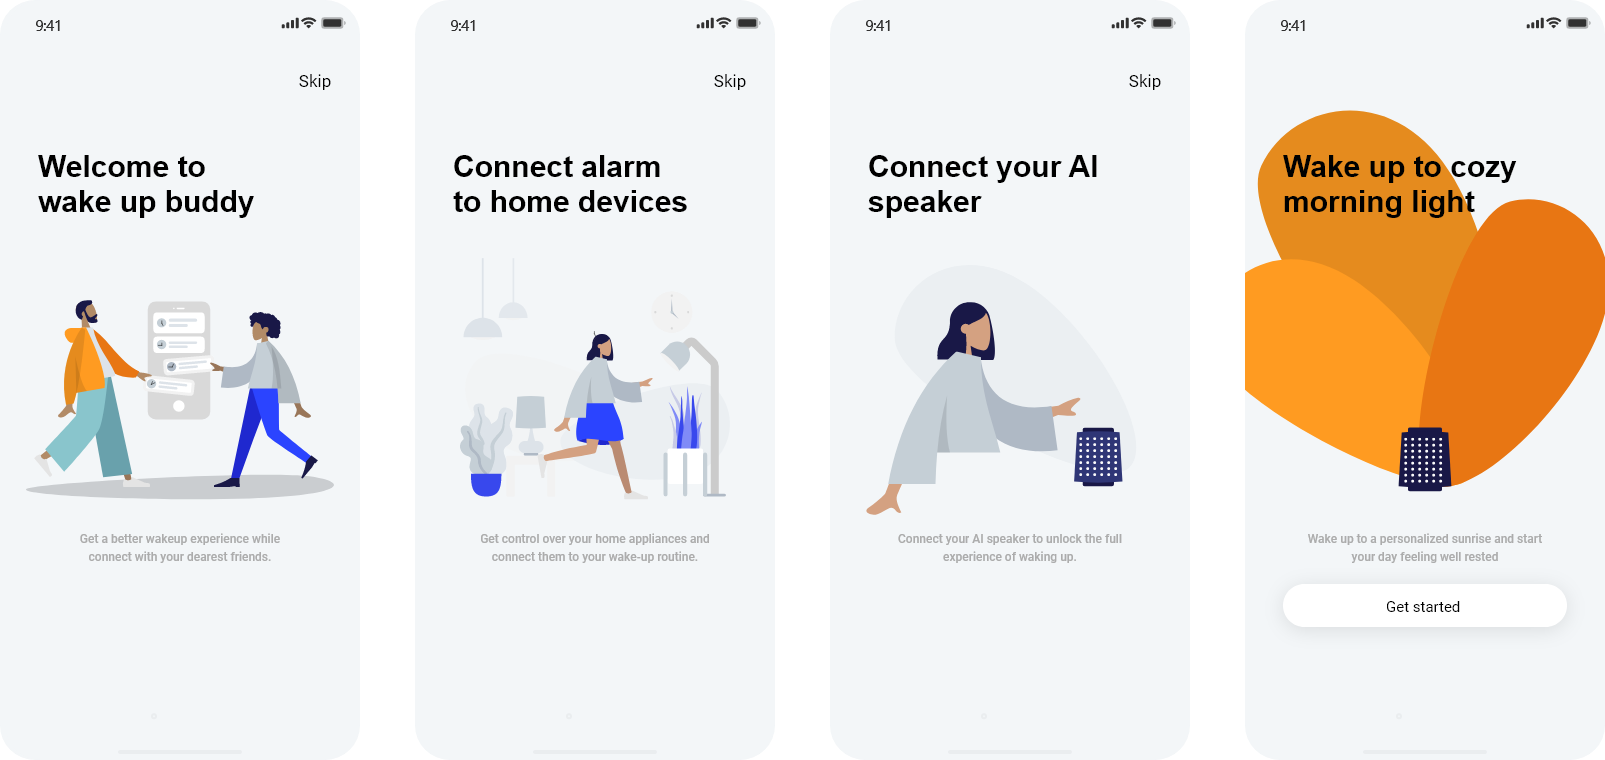
\includegraphics[height=75mm,scale=1]{Images/AppDes.png}}
    \caption{App Description}
    \label{fig}  
\end{figure*}

\subsection{Sign-up/Log-in}
After the logo page the user can sign-up or log in. This window is needed for users to create a new user or enter into the system.
\begin{enumerate}

    \item Log In  \\
    This page consists of two textboxes where users should insert email and password. The “Log in” button is located under these textboxes. If the credentials are wrong the system prompts an error message. If the credentials are correct, the next page is loaded. \par
    If the user has forgotten their password, the user is able to press the clickable text “Forgot password?” which is located under the Login button. on this page users should provide an email address which was indicated earlier during the sign-up process. Under this text field, the button “Send a request” is available to send an email containing the code. The system will pop-up a message if an email is not found in the database.\par
    In addition, log in with an LG account is also available. This is to connect home appliances and applications, which will be described  in the following sections.
    \begin{figure}[htbp]
        \centerline{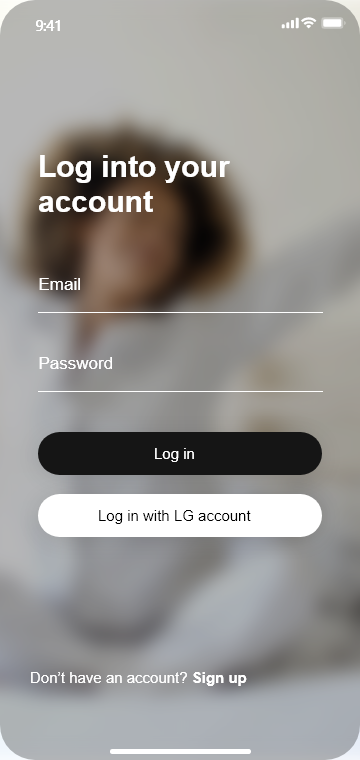
\includegraphics[height=75mm,scale=0.5]{Images/Design_Login.png}}
        \caption{Login Screen}
        \label{fig}
    \end{figure}
    
    
    \item Sign Up  \\
    
   
    It is possible to create a new account by pressing the “Sign up” button. Here, the user provides necessary information such as username, email, and password. For the password textbox, the input characters will be dotted for privacy and at least 5 characters long(has a combination of upper and lowercase letters, numbers, and special symbols). 
    \par Under these three textboxes, there will be a “Sign-up” button in order to create an account and store it in a database for identification. If the user credentials(email and username) are already created, the system warns the user about it, then the user should provide another credential.
    
     \begin{figure}[htbp]
        \centerline{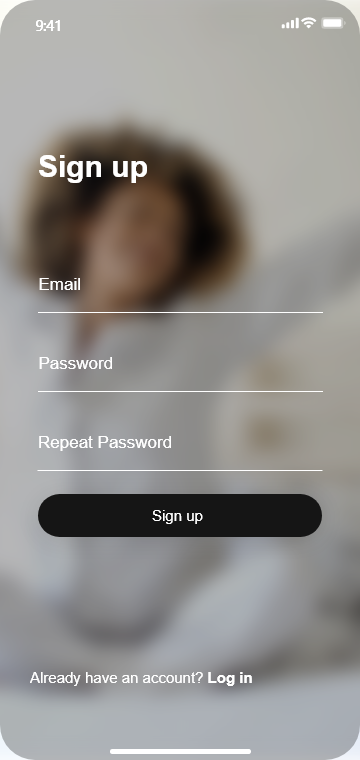
\includegraphics[height=75mm,scale=0.5]{Images/Design_Signup.png}}
        \caption{Sign Up Screen}
        \label{fig}
    \end{figure}
    
\end{enumerate}



\begin{figure*}[!b]
    \centerline{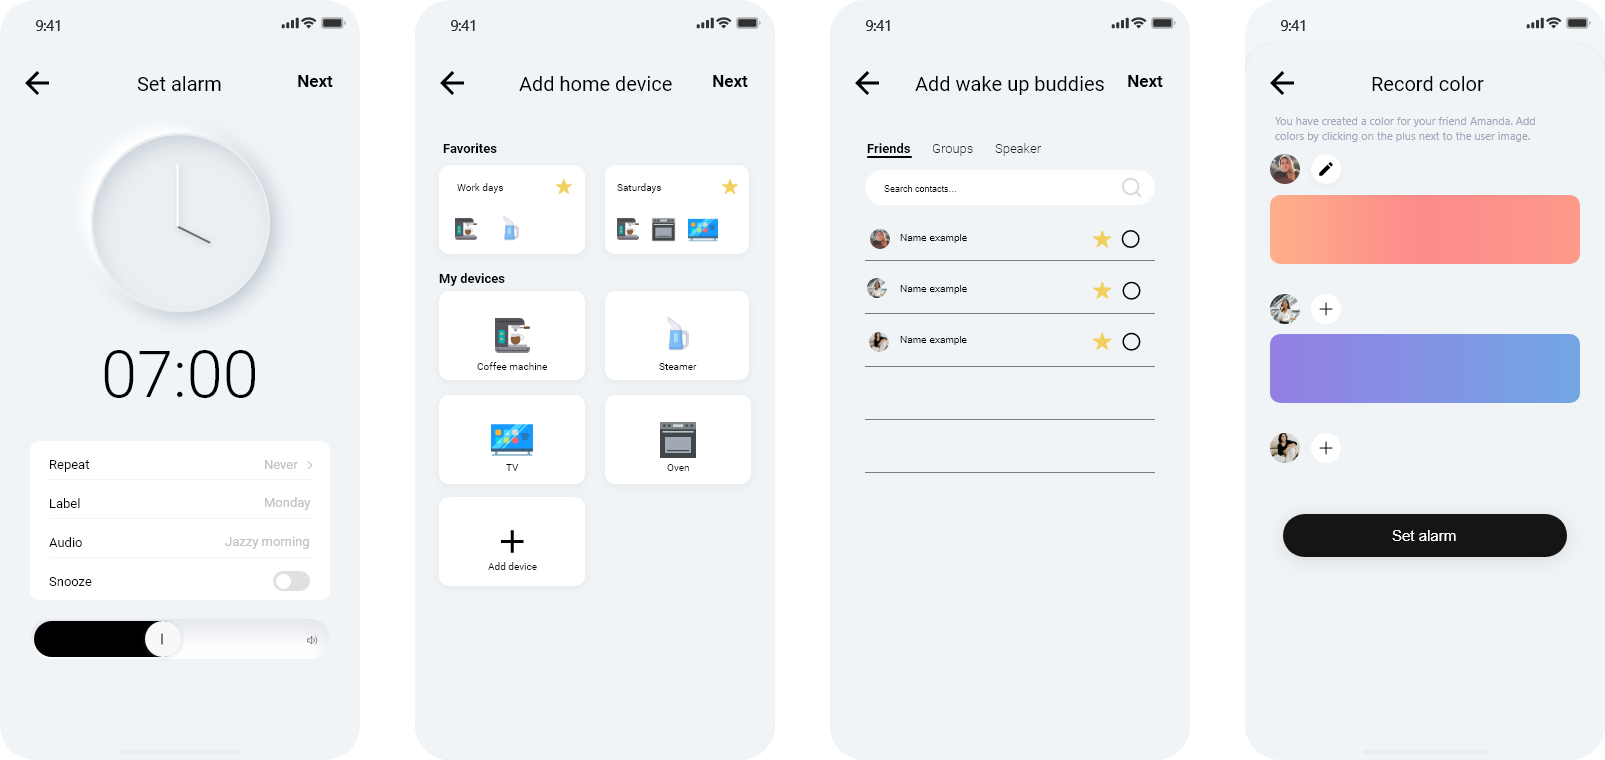
\includegraphics[height=75mm,scale=1]{Images/settingAlarm.png}}
    \caption{Setting an Alarm}
    \label{fig}  
\end{figure*}

\subsection{App description and Setting the initial Settings}
After creating an account or entering the system, the description of this application will be presented before the main page first, and if the user reads it thoroughly, click the GET STARTED button and the next window will appear. The following information is included in the application's description:
\begin{itemize}
    \item “Welcome to wake up buddy”, “Get a better wakeup experience while connect with your dearest friends.”
    \item “Connect alarm to home devices”, “Get control over your home appliances and connect them to your wake-up routine.”
    \item “Connect your AI speaker”, “Connect your AI speaker to unlock the full experience of waking up.”
    \item “Wake up to cozy morning light”, “Wake up to a personalized sunrise and start your day feeling well rested.”
\end{itemize}
After a short tour through the main features of the application, the system should get the information such as date, timezone, and LG account from the operating system.


\subsection{Profile Personalization and Permissions}
After setting the initial settings in the operating system, the user will be guided to give the application access to the camera, location, contacts, storage, and microphone. This can later be changed in the user settings. \par
Lastly, the user has the opportunity to send requests to people from their contacts list and invite those who do not have an account yet.

\subsection{Setting the Alarm/Main page}
\begin{figure}[htbp]
    \centerline{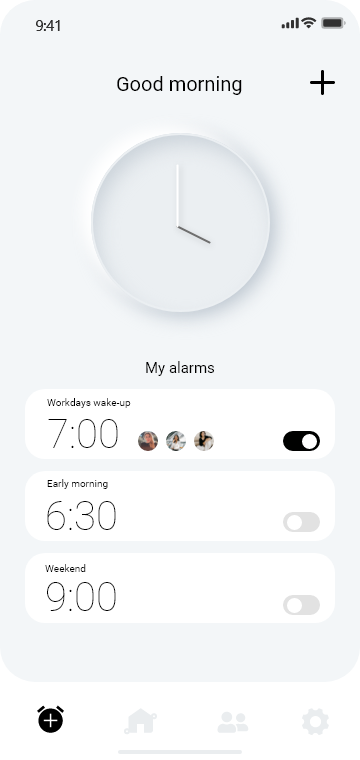
\includegraphics[height=75mm,scale=0.5]{Images/MainPage.png}}
    \caption{Main Page}
    \label{fig}
\end{figure}

The main page displays the alarms. The user can activate an alarm simply by clicking on it. It then changes into an iron color, showing the user that it is activated. The box show relevant information to the user, such as the time of alarm, other members using the same alarm, and the LG home appliances connected to the alarm. If the user wishes to change any specifications of the alarm, they can simply edit the alarm. If there are members included in the alarm, the user is not able to change the time of the alarm. If a user wishes to make a new alarm, they press the button in the bar menu with the icon (+).
\begin{enumerate}
    \item The first step of setting up the alarm is to select the time, and day of the week. If the user wants to wake up every day at the same time, then the user can press the checkbox “Every day”. A way to turn off the alarm, ringer volume, and activation button “Snooze” is accessible. Information about how much time is left before the alarm rings are also available. If the user wishes to end the task, the user can press the “Next” button.
    \item The second step is to add LG home appliances connected to the alarm. It can be a smart lamp, making sure the user wakes up to comfortable lightning. It can be connected to the coffee machine in the kitchen or the styler steaming the outfit for the day. It is also possible to add new appliances if needed. In addition, users can select specific devices as “favorites and save them on the days of the week the user wants them to connect. If the user wishes to end the task at this point, they can press the “Next” button.
    \item The next step is to send out an invitation to friends or add additional home speakers to the alarm. To send out an invitation to a friend, they search for the friend in the search box. User is also able to add chosen contact into “Groups” folder. The invitation is sent out automatically with all settings. An invited person can accept it or reject it. If the user which to attach another home device, for example, a speaker located in one of the children's room, the user can select the speakers the alarm is supposed to be played from. To activate the alarm, the user press the button “set alarm”.
    \item The last step is to add colors by clicking on the "+" next to the user image. The user then can select which color will be displayed on a buddy’s phone or home appliances screen. Here, the user can move their finger to create a personal color recording for a wake-up buddy.

\end{enumerate} \\
Also, in the Main page user can log out from the app.

\subsection{Editing/Deleting an Alarm}
\begin{figure}[htbp]
    \centerline{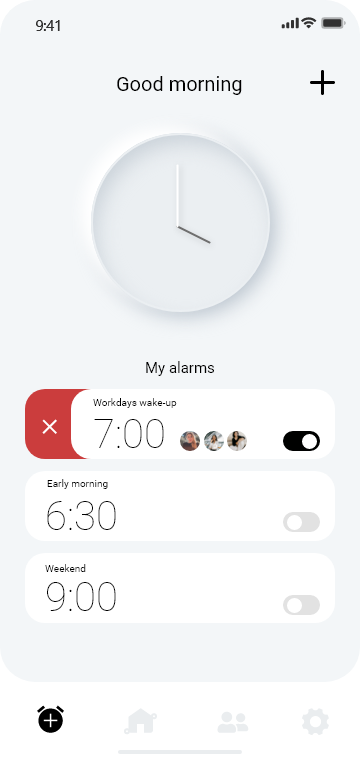
\includegraphics[height=75mm,scale=0.5]{Images/DeletingAlarm.png}}
    \caption{Deleting an Alarm}
    \label{fig}
\end{figure}

On the main page, user selects the alarm which he/she wants to edit.  The user slides the box to the right and a red box appears with a cross. If the user press this box, the alarm is deleted.  When user clicks “Delete” button the system asks the user ”Are you sure you want to delete the alarm?”.  If the user clicks ’Yes’, the alarm is deleted. If the user clicks the blue ’No’, the alarm is not deleted and he or she is returned to the previous page.

\begin{enumerate}
    \item If an alarm is personal, the user can freely edit and delete the alarm. 
    \item If there are other members using the alam, the user can not change the time of the alarm, only regulate the personal home appliances connected to the alarm. If the user wishes to delete the alarm, they can do so and the alarm will be deleted from the local device (not from all devices). 
    \item has unlimited rights with regard to editing and deleting it. It is also possible to send invitations after creating an alarm
\end{enumerate}


\subsection{Report a Person}
\begin{figure}[htbp]
    \centerline{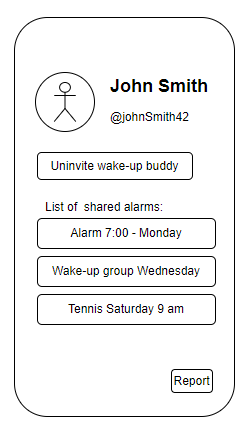
\includegraphics[height=75mm,scale=0.5]{Images/report.png}}
    \caption{Reporting a user}
    \label{fig}
\end{figure}

The user will have the opportunity to report every other user, if he acts in a suspicious/inappropriate way. To do this, the user should open up the profile of the concerned person. Here he will see a report Button called ‘Report’ on which he has to click. On the following page, he will be asked the reason why he thinks the other user should be reported. Therefore, he can choose between different reasons (inappropriate behavior, etc.). In the following time, the report will be reviewed and accepted or declined. In case of acceptance, the reported user will be punished, otherwise, nothing will happen.

    
    
\subsection{Group}
In the group view you can see the name of the alarm, the wake-up time, the username and picture of each member and a chatbox for communication. 
In an additional view, the user can see his personal settings for the regarding alarm. These include among others the sound, vibration (on/off) and the connected LG appliances. This view can only be seen and set by the individual user. 

There are no administrators in a group, all members have the same rights. That is, a group cannot be deleted. Only if every member has left the group, the group will be deleted automatically by the system.

There are the following interaction possibilities in a group:
\begin{itemize}
    \item \textbf{Leave:} Members can leave the group. If they do so, they have the choice of keeping the alert as a personal one.
    \item \textbf{Invite buddies:} Members can invite other people.
    \item \textbf{Post:} members can post messages to the group and other members can respond (with emojis) or comment. Each post and its comments are mapped as a thread. There is an automatic deletion of messages that are older than 24 hours.
    \item \textbf{Mute alarm:} A member can mute the alarm of a group. However, this will be posted in the group.
    \item \textbf{Change group name:} Any member can change the name of the group.\\
\end{itemize}

\subsection{Alarm Notification}
When the set date of the alarm is reached, the alarm notification is triggered. This can look different:
\begin{itemize}
    \item \textbf{Default notification (initially set):} A default ringtone will sound and a default view will be shown with the time and date, a snooze button as well as a stop button. 
    \item \textbf{Custom (additional options to default):} Further, the user can also add today's weather, temperature, news, his own picture or his own message to the default view. He can also set his preferred alarm sound.
    \item \textbf{Wake-up puzzle:} The user can choose to solve a math puzzle, a physical task (sit-ups, push-ups, etc.) or a team building exercise to stop the alarm.\\

\end{itemize}
Regardless of whether the user chooses to snooze or stop, they will then be redirected to the post alert view. This can also look different depending on the alarm type:
\begin{itemize}
    \item \textbf{Not shared alarm:} After the alarm view, the user will be forwarded to the home page of the app.
    \item \textbf{Shared alarm (buddy alarm/group alarm):} After the alarm view, the user will be forwarded to the chat with his wake-up buddy/group chat. Here he has different interaction options: He can send a GIF or an emoji, he can send a typical message or voice message or make a group voice call.\\
\end{itemize}
In the group, the number of snoozes made by a member is displayed. The others have the possibility to react to the 'snoozes' by sending funny sounds or voice messages to the 'still sleeping' member, which will be played automatically at this member.

To improve the experience of waking up, we suggest a physical product to be introduced in the LG home appliances product range. It is a speaker/lamp which could be used together with the alarm. The users can select a color, tune or both for each of the members of the group. When the alarm rings, the color scheme/tunes picked by the user’s friends will play from the lamp and the user can look at the personal color combination made by their friend, knowing that they picked the colors for them. If the user does not have this device, the light will instead come from the screen of the phone and the audio from the phone’s speakers.
This is a way to integrate light into the wake-up experience and at the same time remind the user that they have people thinking of them. 

\subsection{Smart Home Compatibility}
The idea is to give users with LG home appliances a possibility to connect the products to the alarm. The user might want to have their clothes steamed and their coffee made in the mornings. The alarm can automate the task of adapting these systems to the user's wake up time. 

A further version of the app will support the integration with other LG smart home functionalities, such as a connection to a bulb in order to implement a light-based wake up method which simulates the sunrise or a connection to the shutters to actually be woken by the sun. 
The above applications can be selected when creating an alarm clock. However, the app must first be linked to a LG account. If the desired LG home appliances are linked to this account, they are also available in the alarm.

Additionally, the app can be further developed to support AI assistants so that it can support hands-free control of the app by taking voice commands.

\subsection{Monitoring}
The data, which accumulates over time, is stored, analyzed and presented to the user. There will be a separate tab for this. In addition to the average wake-up time, the average number of snoozes and the most popular wake-up buddies of the user, meta-data will also be collected, such as which wake-up buddies make getting up the easiest (measured by the number of snoozes).\\

\section{Architecture Design \& Implementation}
\subsection{Overall Architecture}
Wake Up Buddy is divided into 7 main modules which interact together to deliver the features of the app.

\begin{figure}[htbp]
    \centerline{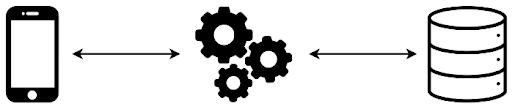
\includegraphics[height=15mm,scale=0.5]{Images/architecture_brief.png}}
    \caption{Overall Architecture}
    \label{fig}
\end{figure}
    
\begin{figure}[htbp]
    \centerline{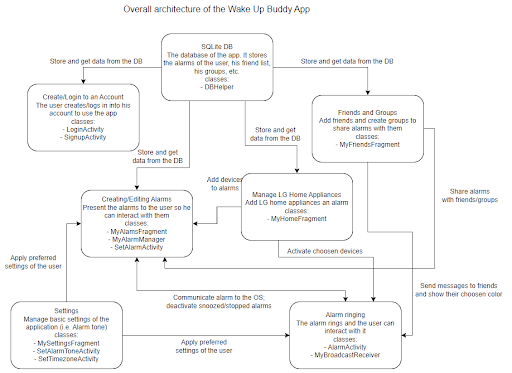
\includegraphics[height=75mm,scale=0.5]{Images/architecture.png}}
    \caption{Detailed Architecture}
    \label{fig}
\end{figure}
    
\subsection{Directory Organization}
The following table shows the directory structure of the Git Repository

\begin{table}[h]
\caption{Directory Structure of the Git Repository}
\def\arraystretch{1.24} \small
    \begin{tabular}{|p{2.6cm}|p{5.0cm}|}
	\hline
	Directory & Contents\\
      \hline
       /WakeUpBuddy & Root directory with .gitignore and Readme file \\
	\hline
        /WakeUpBuddy/ Documentation & Documentation in a pdf file format and as a latex file\\
	\hline
        /WakeUpBuddy/ DB\_SQLite & SQLite Database and SQL scripts\\
	\hline
	/WakeUpBuddy/src/ App & Root directory for the Android application. It contains the gradle scripts and the further directories .\\
    \hline
    /WakeUpBuddy/src/ App/app/src/main & Place of the AndroidManifest file. \\
    \hline
	/WakeUpBuddy/src/ App/app/src/main/ java/com/example/ wakeupbuddy & Main directory for the kotlin source code of the Android app. Every source code file which is not representing an activity, fragment or model is stored in this directory.\\

    \hline
    …/com/example/ wakupbuddy/activities & Folder that bundles all kotlin classes which are use as activities by the app. \\
    \hline
    …/com/example/ wakupbuddy/fragments & Directory that bundles all kotlin classes which are interpreted as fragments by the compiler. \\
    \hline
    …/com/example/ wakupbuddy/models & Folder that contains all kotlin data classes/models of the project. These are used to reach a consensus of how the data of the database and the app is structured. \\
    \hline
    /WakeUpBuddy/src/ App/app/src/main/ res & Directory where the xml files are stored. These will be later presented as the layout of the map. It also contains everything else which will be later presented on the smartphone screen. \\
	\hline
	\end{tabular}
\end{table}   

\subsection{Module 1: Create/login to an account}


\begin{enumerate}
    \item Purpose: \\
        The purpose of this module is to manage user accounts: create or log in. These data are stored and taken from the database. If the user does not have an account yet, he can create one and then log in with it again and again. Here the simplest logical checks are performed. To be more precise, user is not available to duplicate emails and usernames. Also, password and confirmation password must match. None of the other features can be used if the user is not logged in.\\ 

    \begin{figure}[htbp]
        \centerline{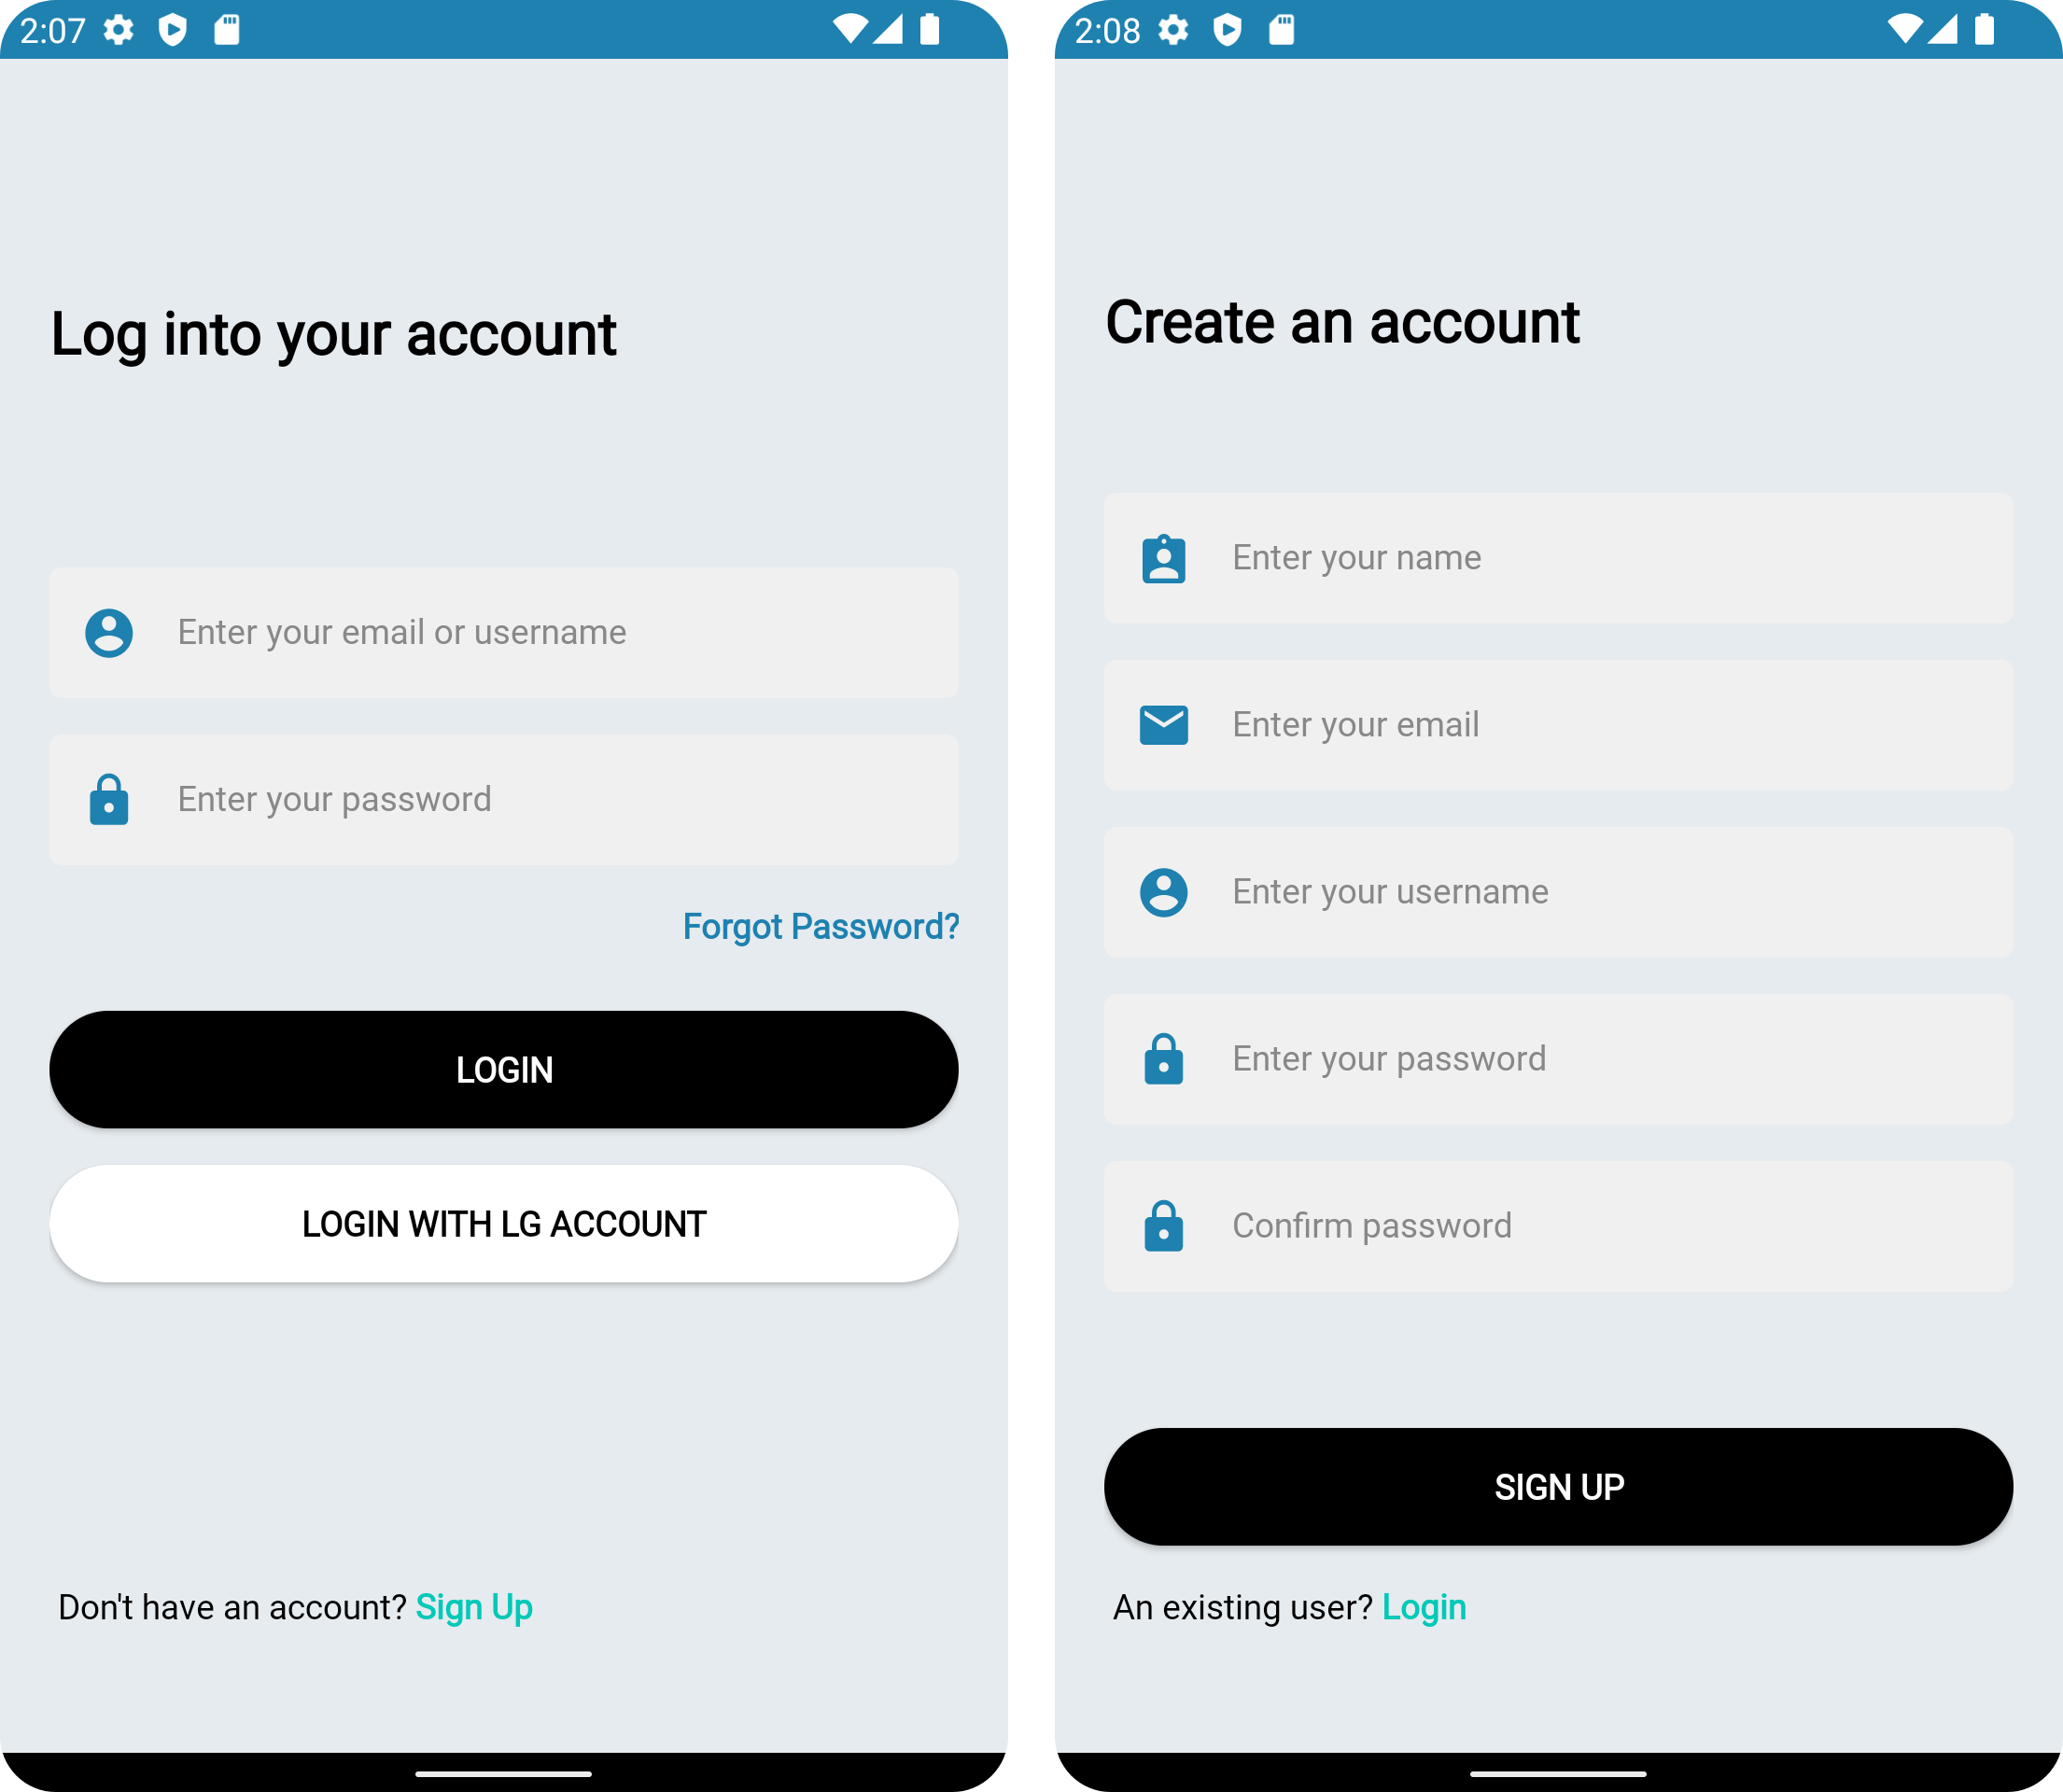
\includegraphics[height=65mm,scale=0.5]{Images/App_Login_Signup.png}}
        \caption{Login / Signup Pages}
        \label{fig}
    \end{figure}
    
    \item Functionality: 
    \begin{itemize}
        \item Gets the login and passwords through DBHelper from the database.
        \item Any changes in username and password will be edited in a database.
        \item  Checks if the credentials are wrong during login then the system prompts an error message. If not, the next page will be presented.
        \item  If the user has forgotten their password, the user is able to press the clickable text “Forgot password?”
        \item Creates a new account by pressing “Sign up” button.
    \end{itemize} 
    \item Location of Source Code:
    \begin{itemize}
        \item /WakeUpBuddy/src/App/app/src/main/java/com/
        example/wakeupbuddy/activities/
    
    \end{itemize} 
    \item Class Components:
    \begin{enumerate}
        \item LoginActivity \\
            LoginActivity class represents the way how user log in to the system using required credentials.
        \item SignupActivity \\
            This class shows the logic for creating a new account and forms the backend for the Signup Activity. 
        
    \end{enumerate}
\end{enumerate}

    \begin{figure*}[!b]
        \centerline{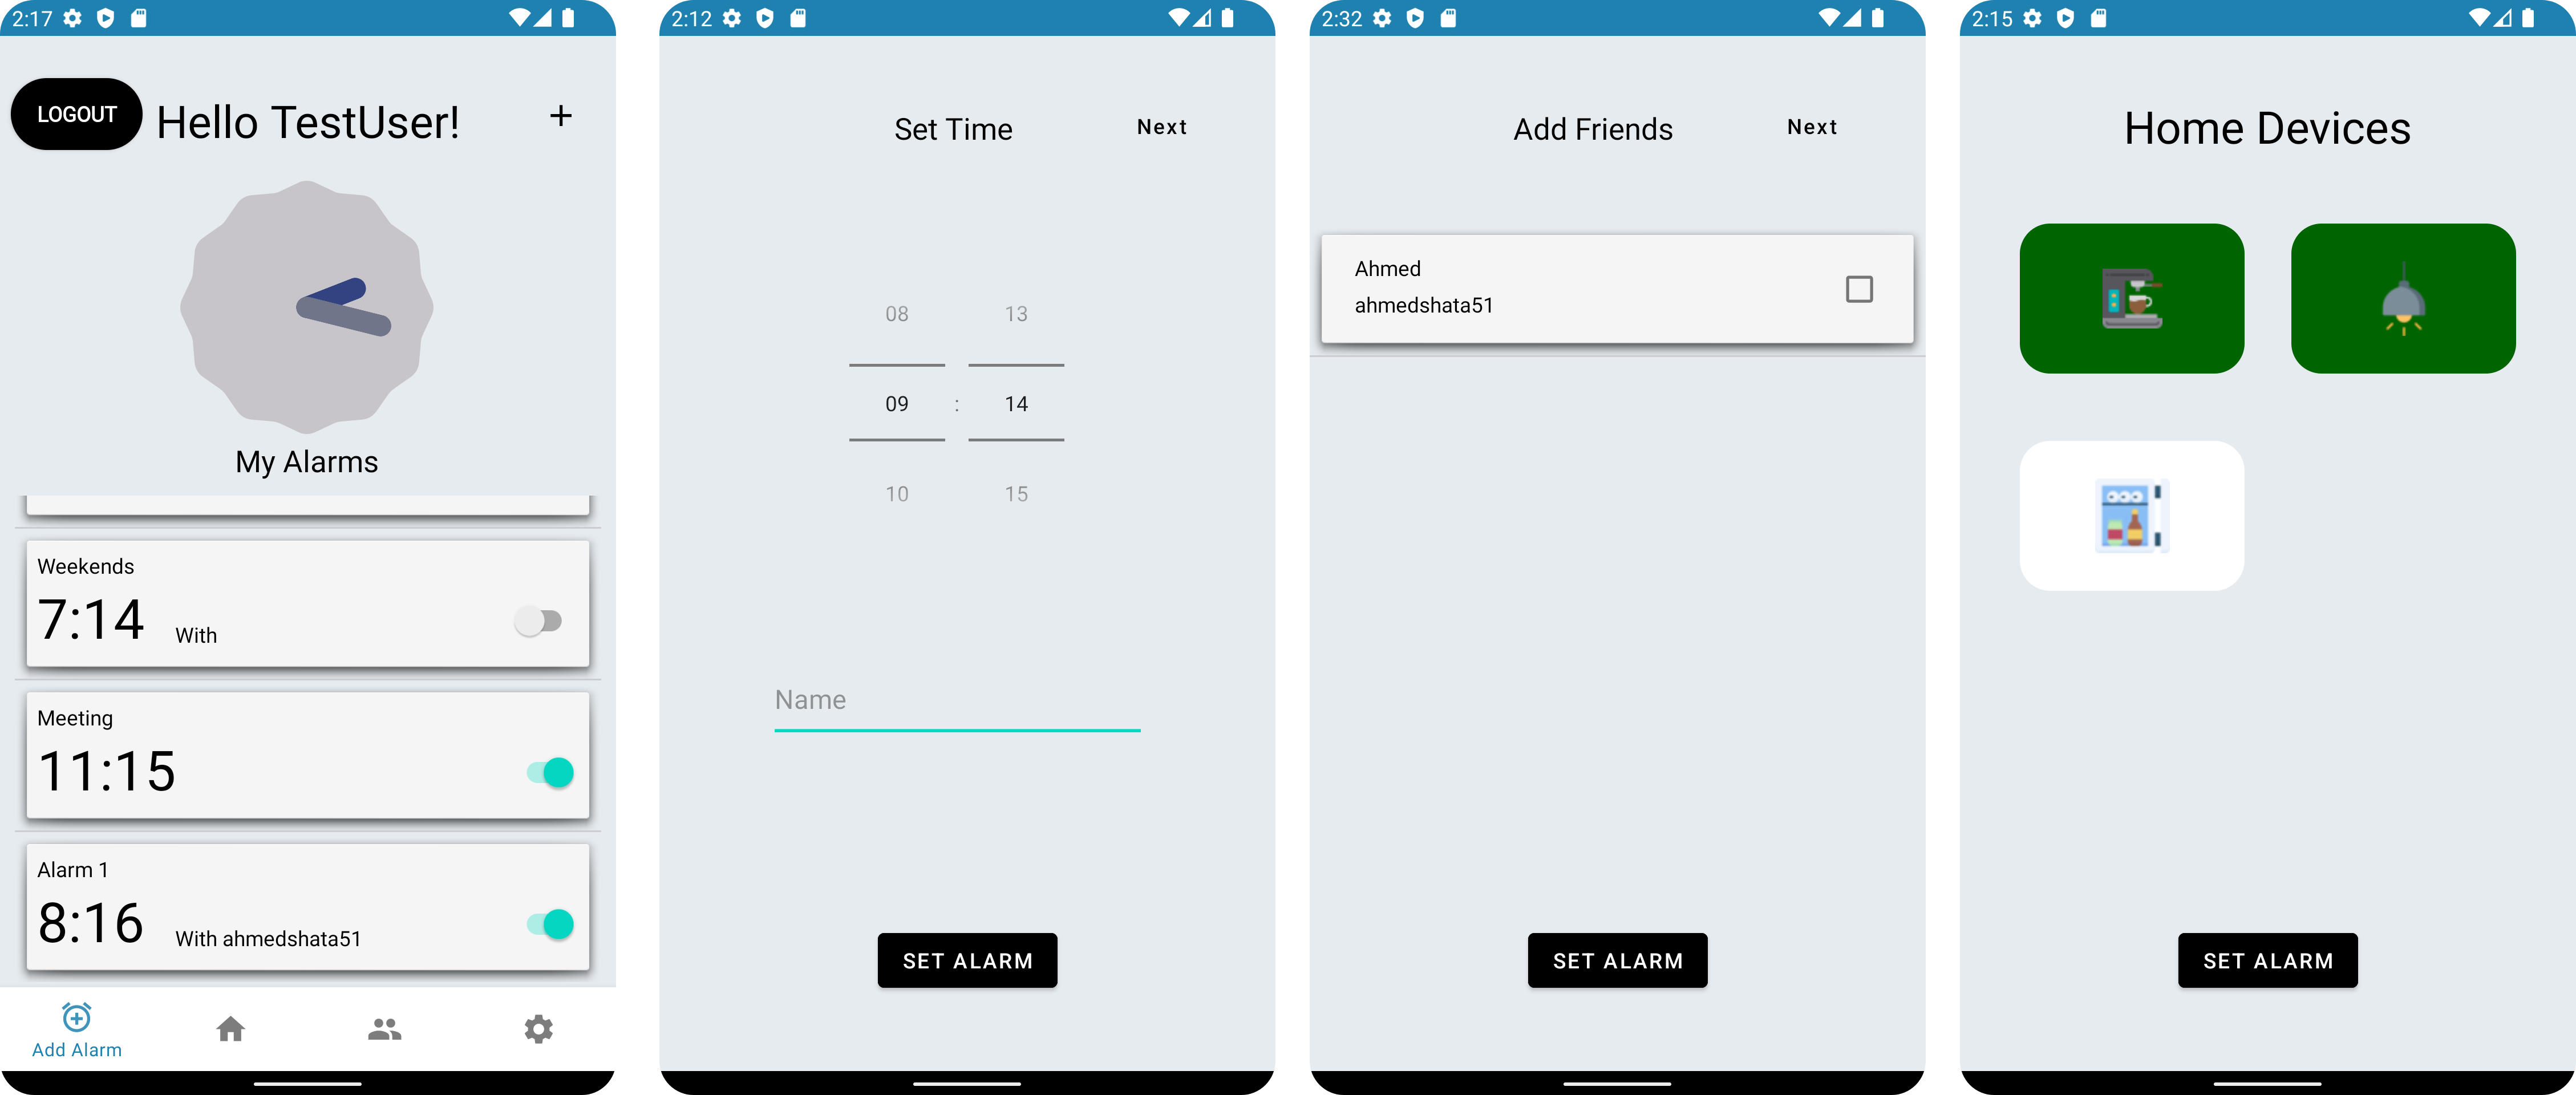
\includegraphics[height=75mm,scale=0.8]{Images/App_SettingAlarm.png}}
        \caption{Setting an Alarm in the app}
        \label{fig}  
    \end{figure*}
\subsection{Module 2: Creating/Editing Alarms}
\begin{enumerate}
    \item Purpose: \\
    This is the central module of the application. It manages the user's alarms in one place. These are retrieved from the database at the start of the application and stored in a dynamic list. This is then presented to the user, who can now interact with it. For example, if he creates a new alarm via the app's layout, it is first added to the list and then stored in the database. 
    \par The interaction of other modules/components of the app must also use the Alarm Manager if they want to access or manipulate the alarm.\\ 

    \item Functionality: 
    \begin{itemize}
        \item gets the alarms via DBHelper from the database
        \item manages the alarms in a dynamics list
        \item manages activation/deactivation of alarms
        \item manages creation/editing/deletion of alarms
        \item works as proxy for other modules that want to access an alarm
    \end{itemize} 
    \item Location of Source Code:
    \begin{itemize}
        \item /WakeUpBuddy/src/App/app/src/main/java/com/example/ wakeupbuddy
        \item /WakeUpBuddy/src/App/app/src/main/java/com/example/ wakeupbuddy/Activities/
        \item /WakeUpBuddy/src/App/app/src/main/java/com/example/ wakeupbuddy/Fragments/
        \item /WakeUpBuddy/src/App/app/src/main/java/com/example/ wakeupbuddy/Models/
    \end{itemize} 
    \item Class Components:
    \begin{enumerate}
        \item MyAlarmManager: \\
            This class serves as a central point to manage the user's alarms. These, after being loaded from the database to start the application, are stored and managed in a dynamic list. 
            \par The class serves in parallel as a Customized Adapter, a derived class of the BaseAdapter class. This means that the instance of MyAlarmManager with the list of alarms, is made available to the operating system so that it can render the alarms for the layout that is displayed to the user.
            \par In addition, the class also acts as a proxy for other modules of the application that want to access the list of alarms. Thus, no alarms can be created or deleted directly or stored in the list. This must happen via a getter / setter function of the MyAlarmManager class. 
            \par For example, there is the "createAlarm" function, which takes the time of the desired alarm as a parameter and instantiates an object of the AlarmModel class from this data. It then appends this to the list of alarms and communicates to the operating system that a broadcast is to be sent at the corresponding time. This is then intercepted by the MyBroadcastReceiver class, whereupon the alarm sounds.
            \par Furthermore there are two functions to activate or deactivate a desired alarm. These map the switch button of the overlay. When loading the layout, it is read from the respective instances of the AlarmModel classes whether the alarm should be displayed as activated/deactivated and this is displayed in the layout as a marked/unmarked switch button. With the help of an onSwitchListener now each change of this state is registered by the user and stored back into the alarm object. In parallel, a broadcast event is started if the alarm is activated, or canceled if the alarm is deactivated. Since the MyAlarmManager class is used as a proxy, the Alarm ringing module can also access the deactivation function. In this case, the alarm sound that sounds when the alarm is active will also be stopped.\\
        \item MyAlarmsFragment: \\
            This class represents the backend or logic for the MyAlarms fragment of the application. This presents the list of alarms to the user. It is the first page he sees after logging in. Here he is given the possibility to create additional alarms or interact with already created alarms, for example, activate/deactivate them.
            \par The particular logic to be executed when the user presses a button is defined in onClickListeners in this class. \\
        \item SetAlarmActivity: \\
            This class encapsulates the logic for creating alarms and thus forms the backend for the SetAlarm activity. The time of the alarm as well as the rest of the information is defined here by the user and then passed to the createAlarm function of the MyAlarmManager class. \\
        \item AlarmModel:
            This class is a simple data class of Kotlin. It is used to map the alarm table of the database as a class and thus simplify the interaction between them. \\
        
    \end{enumerate}
\end{enumerate}

\subsection{Module 3: Alarm Ringing}

\begin{enumerate}
    \item Purpose: \\
    When the alarm sounds for the user, this module is active. It implements the various activities around the ringing of the alarm.\\ 
    
    \begin{figure}[htbp]
        \centerline{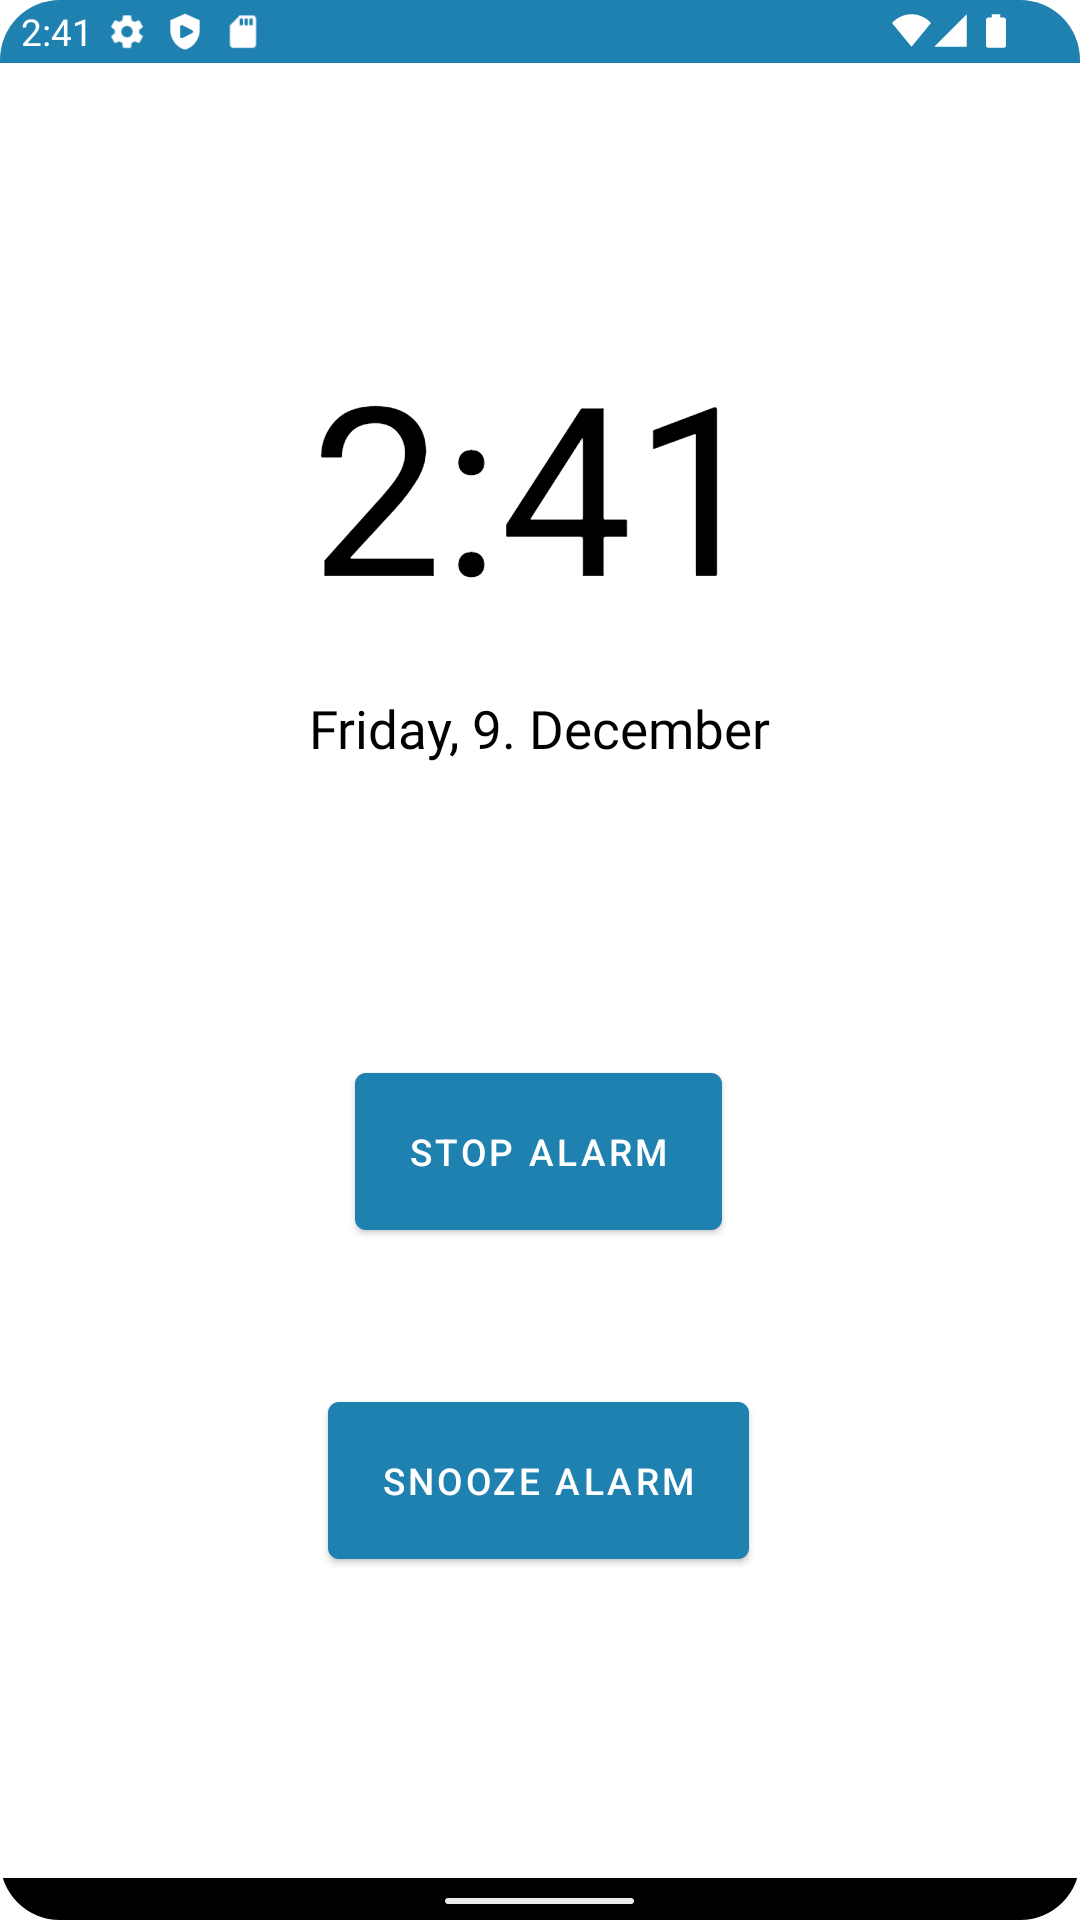
\includegraphics[height=65mm,scale=0.5]{Images/App_AlarmRinging.png}}
        \caption{Alarm Notification}
        \label{fig}
    \end{figure}
    
    \item Functionality: 
    \begin{itemize}
        \item Catch Broadcast from the Operating System and start the alarm.
        \item Present the alarm and all of its features according to the settings to the user.
        \item Communicate the stop or snooze action of the user to the MyAlarmManager instance.
    \end{itemize} 
    \item Location of Source Code:
    \begin{itemize}
        \item /WakeUpBuddy/src/App/app/src/main/java/com/
        example/wakeupbuddy/
        \item /WakeUpBuddy/src/App/app/src/main/java/com/
        example/wakeupbuddy/Activities/
    \end{itemize} 
    \item Class Components:
    \begin{enumerate}
        \item MyBroadcastReceiver \\
            This class is derived from Android's BroadcastReceiver and receives the alarm event. This is fired by the operating system when the previously set time of the alarm is reached.
            \par Then this class starts the alarm activity, which includes the user's preferred alarm sound and vibration if they have been marked as enabled in the Settings object. \\
        \item AlarmActivity \\
            This class encapsulates the logic of the alarm activity. The activity presents the user with a familiar stop/snooze interface that allows him to stop or snooze the alarm. At the same time, he is also shown other details, such as the current time or the weather. If the user decides to click on the Stop or Snooze button, a previously initialized onClickListener is activated, which executes the corresponding logic. 
            \par Basically, the logic of the Stop and the Snooze functionality does not differ much. In both functions, the current alarm is first disabled, so the alarm sound and vibration (if on) are turned off. Then the activity is stopped and the user is redirected to the MyAlarms fragment. At the same time, when snoozing, a new alarm event with the time of the alarm plus five minutes is communicated to the operating system. On the other hand, when the alarm is stopped, this does not happen. Instead, the alarm event for the next day is sent to the operating system.\\
        
    \end{enumerate}
\end{enumerate}

\subsection{Module 4: Manage LG Home Appliances}
\begin{enumerate}
    \item Purpose: \\
    The purpose of this module is to select to which home appliances connect the user's alarm.  This module contains data related to home appliances management. The user should choose one or more desired appliances. For example, if user wants to wake up with the coffee ready, user can connect the coffee machine to the alarm.\\ 

    \item Functionality: 
    \begin{itemize}
        \item Manages activation of chosen by user home appliances.
        \item Connects LG’s devices to the current account of the user.
    \end{itemize} 
    \item Location of Source Code:
    \begin{itemize}
        \item /WakeUpBuddy/src/App/app/src/main/java/com/
        example/wakeupbuddy/fragments/
        \item /WakeUpBuddy/src/App/app/src/main/java/com/
        example/wakeupbuddy/Activities/
    \end{itemize} 
    \item Class Components:
    \begin{enumerate}
        \item MyHomeFragment \\
            This is the third-page user sees after creating the alarm and adding the friends. This class presents the list of appliances to the user.  Also, this class shows the backend for the MyHomeFragment. In this fragment, the user is given the possibility to choose appliances from the list which is already created, so no availability to create additional home appliances. \\
        
    \end{enumerate}
\end{enumerate}

\subsection{Module 5: Friends and Groups}

    
\begin{enumerate}
    \item Purpose: \\
        The aim of this module is to be able to create a group to share alarms with them. It consists of a friends list in a database in order to choose from and create a group. This is the first page after creating the alarm, so the user can decide whether to apply this alarm to the user’s friends too. If yes, friends get a notification about the alarm.
        \par In order to share the alarm with the buddies the user must first add them as a friend so that they can then be selected when creating the alarm. When adding, a group of the selected friends including the selecting user is created in the background and added to the alarm. Here, it is also available to select buddies as “favorite” ones, so the user does not select one person each time, this buddy is located in a “favorite”, so it is easier for the user to select.\\ 
        
    \begin{figure}[htbp]
        \centerline{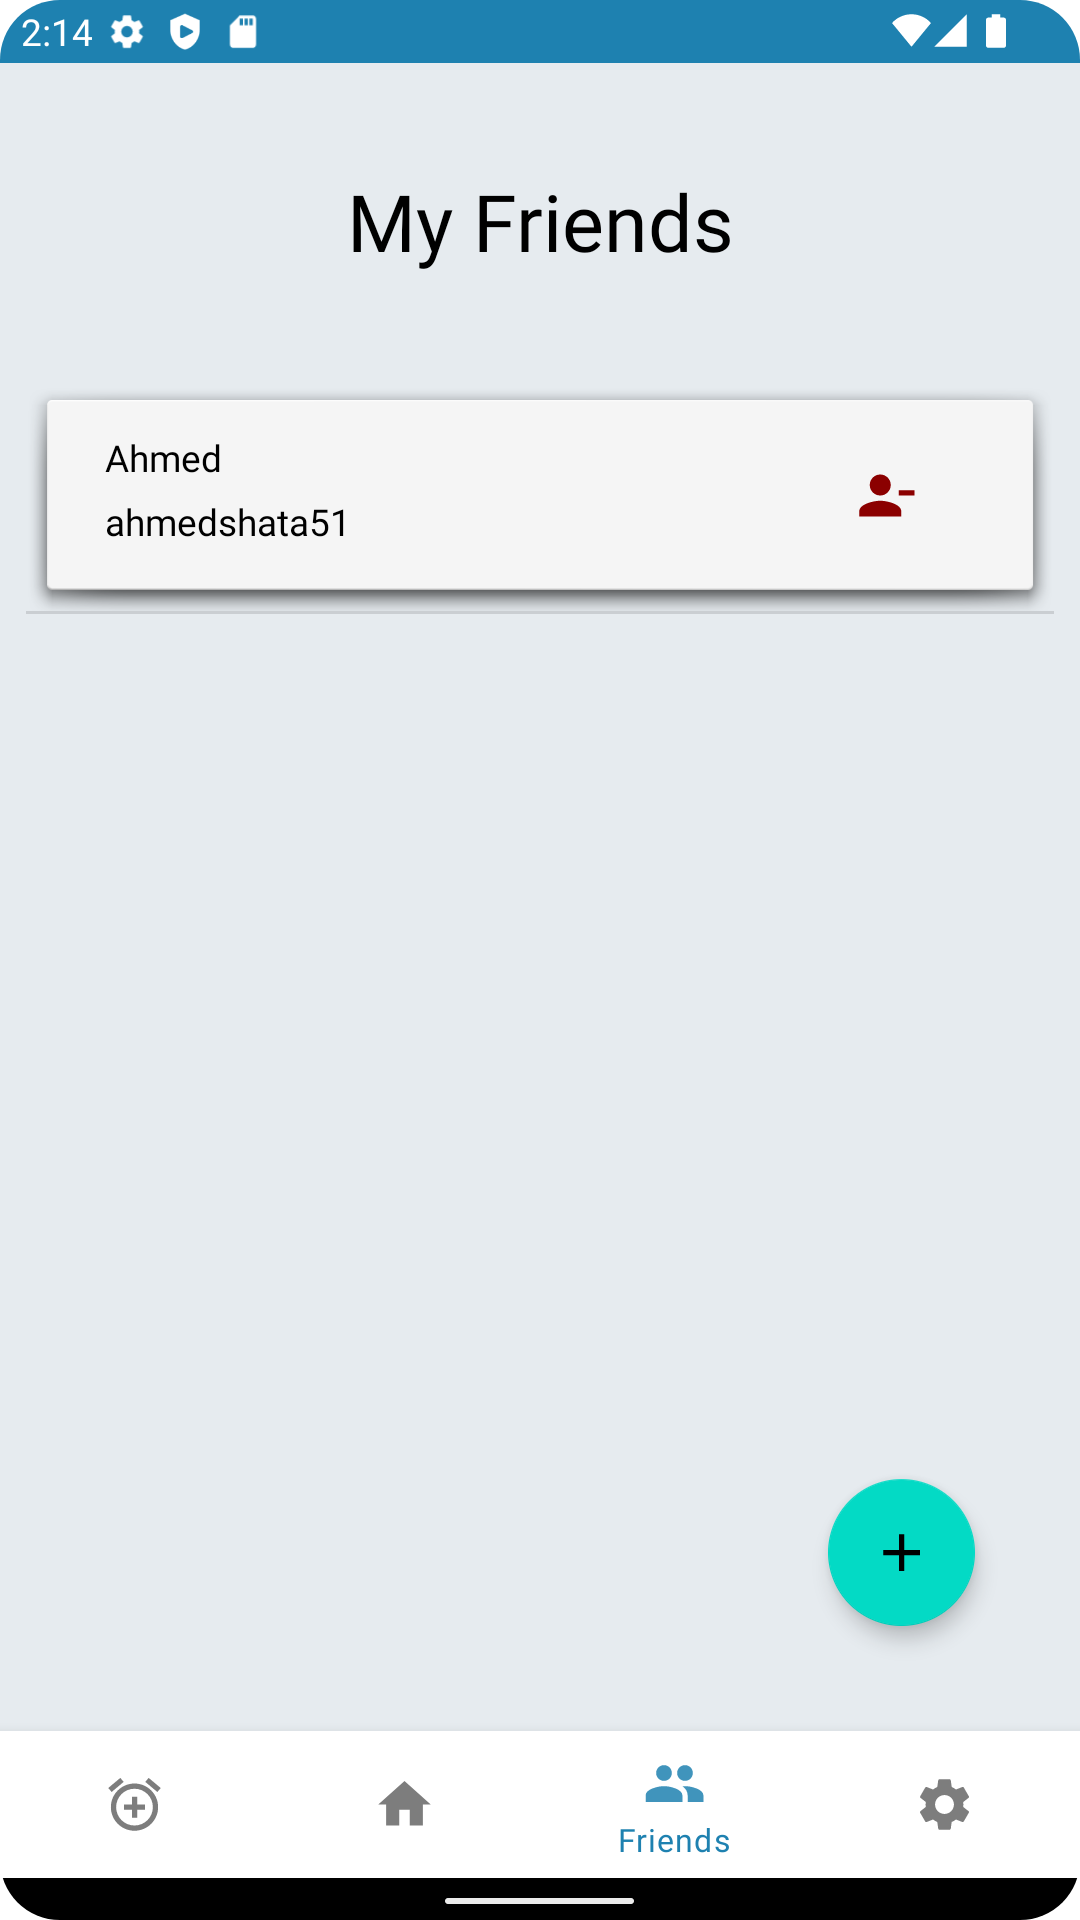
\includegraphics[height=65mm,scale=0.5]{Images/App_MyFriends.png}}
        \caption{Adding Friends}
        \label{fig}
    \end{figure}
    
    \item Functionality: 
    \begin{itemize}
        \item Gets the friends list via DBHelper from the database.
        \item Enable the “favorite” list, so the user can select from the favorite list.
        \item No administrator, so the group can’t be deleted and it enables equal rights in a group
        \item It is possible to leave the group so the user can save the alarm as a personal one.
        \item Allows to invite friends
    \end{itemize} 
    \item Location of Source Code:
    \begin{itemize}
        \item /WakeUpBuddy/src/App/app/src/main/java/com/
        example/wakeupbuddy/fragments/
        \item /WakeUpBuddy/src/App/app/src/main/java/com/
        example/wakeupbuddy/models/
    \end{itemize} 
    \item Class Components:
    \begin{enumerate}
        \item AddFriendsActivity \\
        This class represents the logic behind adding friends for an alarm. Through this activity, the user is provided a search interface with the help of which the user can be able to make searches within the given list of buddies. The user has to enter the search query in this search view. The listview will be filled with the query results based on the search.
        \item MyFriendFragment \\
            This forms the backend for the MyFriendFragment. Here, user can search for a friend from the whole list or search the friend from the “favorite” list. 
        \item FriendConnectionModel \\
        This class is a simple modal class for storing the friends ID. 
        
    \end{enumerate}
\end{enumerate}


\subsection{Module 6: Settings}
\begin{enumerate}
    \item Purpose: \\
    The purpose of this module is to manage the user's preferences bundled in one place and stored locally. The user should be able to shape his wake-up experience in the way that is most pleasant for him. For this purpose, he can, for example, switch the vibration of the smartphone on and off when the alarm sounds or change the ringtone. Afterwards, the values are persisted, so that the user does not have to set them every time.\\ 
    \begin{figure}[htbp]
        \centerline{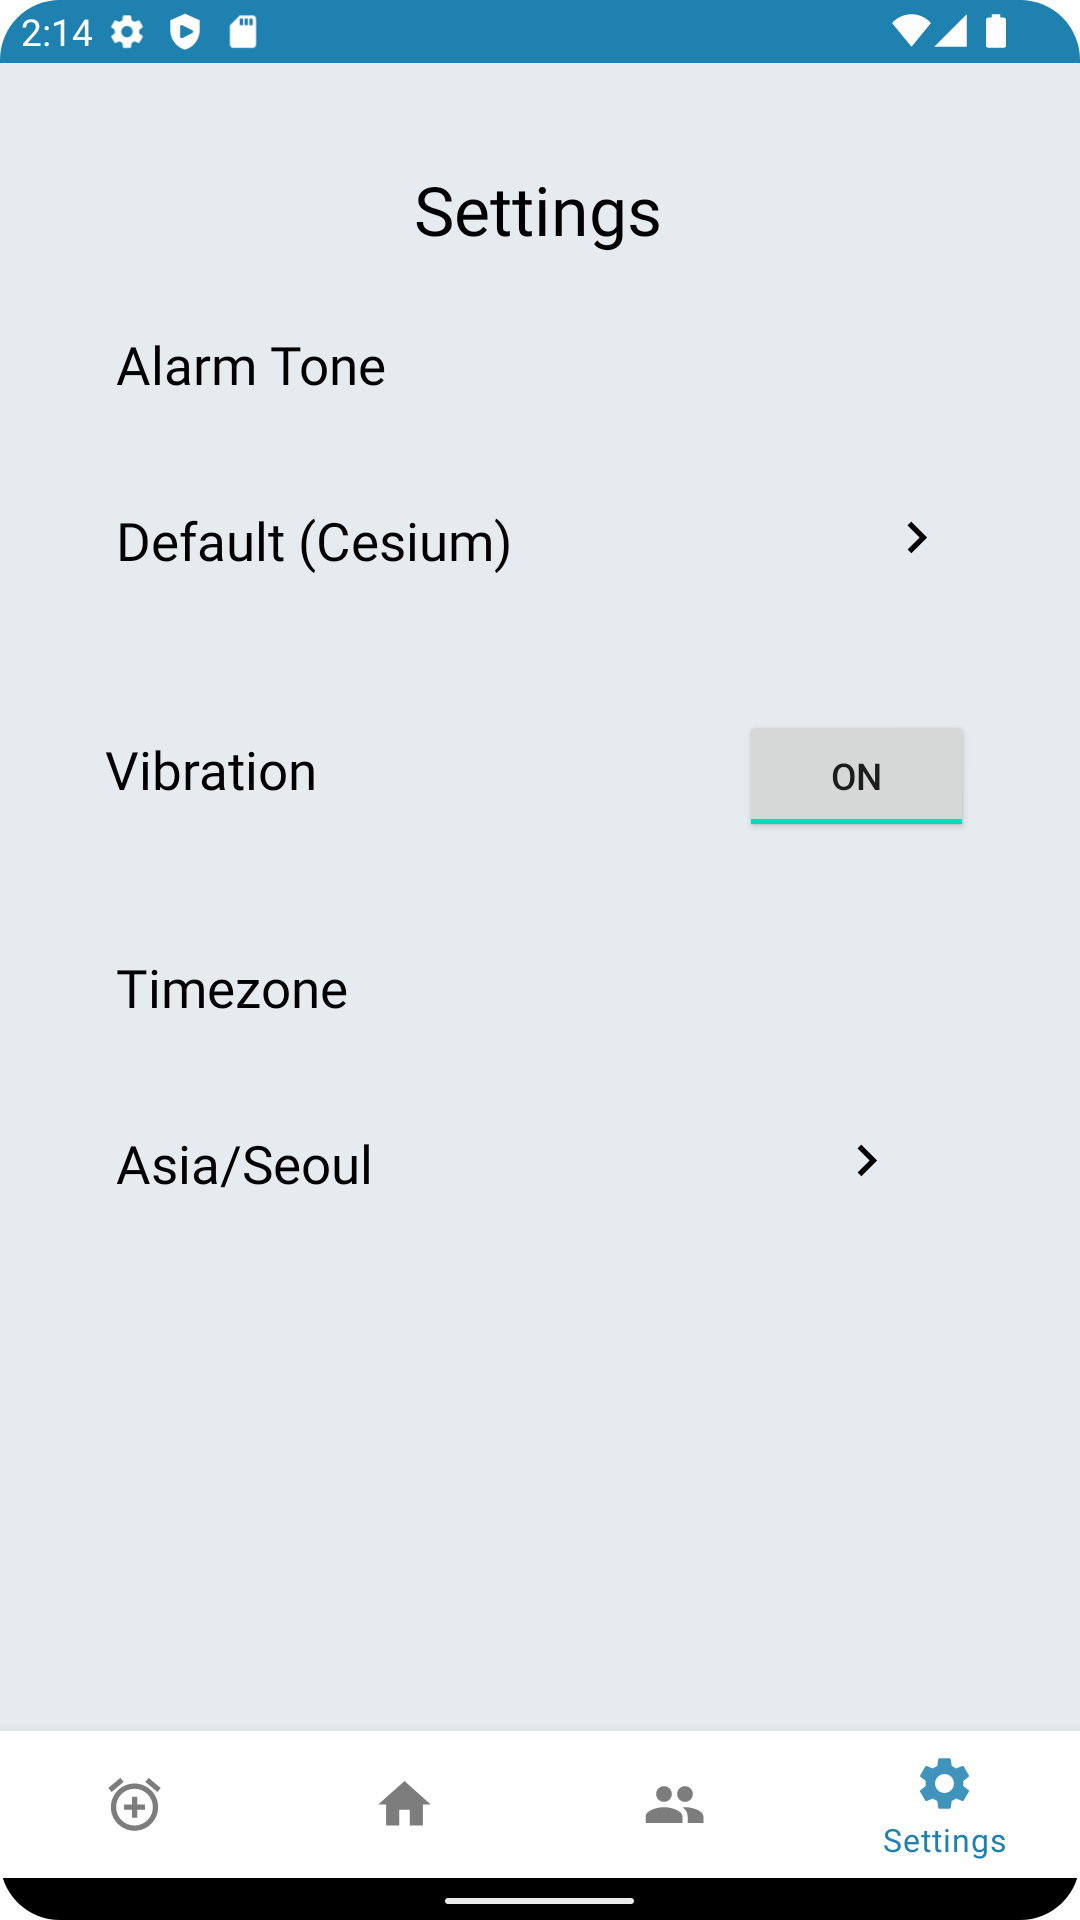
\includegraphics[height=65mm,scale=0.5]{Images/App_Settings.png}}
        \caption{Settings Page}
        \label{fig}
    \end{figure}
    
    \item Functionality: 
    \begin{itemize}
        \item persist preferences of the user beyond the time the app runs
        \item enable changing of the alarm tone, vibration and timezone
    \end{itemize} 
    \item Location of Source Code:
    \begin{itemize}
        \item /WakeUpBuddy/src/App/app/src/main/java/com/example/ wakeupbuddy/Activities/
        \item /WakeUpBuddy/src/App/app/src/main/java/com/example/ wakeupbuddy/Fragments/
        \item /WakeUpBuddy/src/App/app/src/main/java/com/example/ wakeupbuddy/Models/
    \end{itemize} 
    \item Class Components:
    \begin{enumerate}
        \item SettingsFragment: \\
            This class forms the backend for the Settings fragment. This presents the settings of the user, so that he can make changes. Among other things, the fragment presents the currently used alarm sound and the currently used time zone. In addition, the fragment displays whether the alarm should take place with vibrations.
            \par If the user decides to change something in these settings and clicks on the corresponding button, the previously set onClickListener is activated and either forwards the user to the next activity or applies the changes directly (in the case that no further user interaction is required).
            \par The settings are dynamically managed in an instance of the SettingsModel class and persisted over the runtime of the application using the SharedPreference class. This means that the data is stored in a file locally on the user's smartphone. Each time the application is launched, the settings from the file are loaded into an instance of the SettingsModel class and meanwhile managed there. If a setting is changed, it is also changed or stored directly in the file in parallel with the instantiated object. \\
        \item SetAlarmToneActivity \\
            This class contains the logic for the SetAlarm activity. In it, the user can choose from the various default alarm tones of the smartphone the tone they want to hear when the alarm goes off. The list of alarm tones is implemented using the same principle as the list of alarms in the MyAlarmManager class, with a ListView in the XML file and a derived custom adapter with a list. When the activity is started, the list is initialized with all the default tones of the operating system.
            \par Once it has decided on a tone, it is stored as a combination of name and URI in the SettingsModel object and the file. \\
        \item SetTimezoneActivity \\
            As with the SetAlarmToneActivity class, the SetTimezoneActivity class forms the backend for the SetTimezone activity. If the user decides to change the timezone, he will be presented with all possible timezones from which he can then choose his preferred zone.
            \par As with selecting an alarm tone, a ListView in combination with an adapter is used to present the time zones. \\
        \item SettingsModel \\
            This class is a simple data class of Kotlin. It is used to keep the settings bundled in one class and make them accessible to all other modules/classes in a unified way. \\
        
    \end{enumerate}
\end{enumerate}

\subsection{Module 7: SQLite DB}
\begin{enumerate}
    \item Purpose: \\
    Stores the alarm of the user, his friends list, group, home appliances. A temporary dataset processed with some data in an application using SQLite.\\ 

    \item Functionality: \\
        \begin{itemize}
            \item In this class you can create, delete, or edit DB entries
            \item Storage of relevant data like users, groups or alarms is managed
        \end{itemize}
    \item Location of Source Code:
    \begin{itemize}
        \item WakeUpBuddy/src/App/app/src/main/java/com/
        example/wakeupbuddy/DBHelper.kt
    \end{itemize} 
    \item Class Components:
    \begin{enumerate}
        \item DBHelper \\
            This class is basically our interface between the DB and our application. Via models you communicate with the DB and get also results as Lists or single model elements. 
            \par In this class you can create, delete, or edit DB entries.
        \item WakeUpBuddyApp \\
        is accessible from every module/class and thus forms a central point for the storage of data and the interaction between the modules.
    \end{enumerate}
\end{enumerate}
\vspace{10pt}
\section{Use Cases}
\begin{enumerate}
    \item Sign up/ log in: \\
        In order to use the application, the user needs an account. The user can log in with their LG account or create a new account.
        \begin{figure}[htbp]
            \centerline{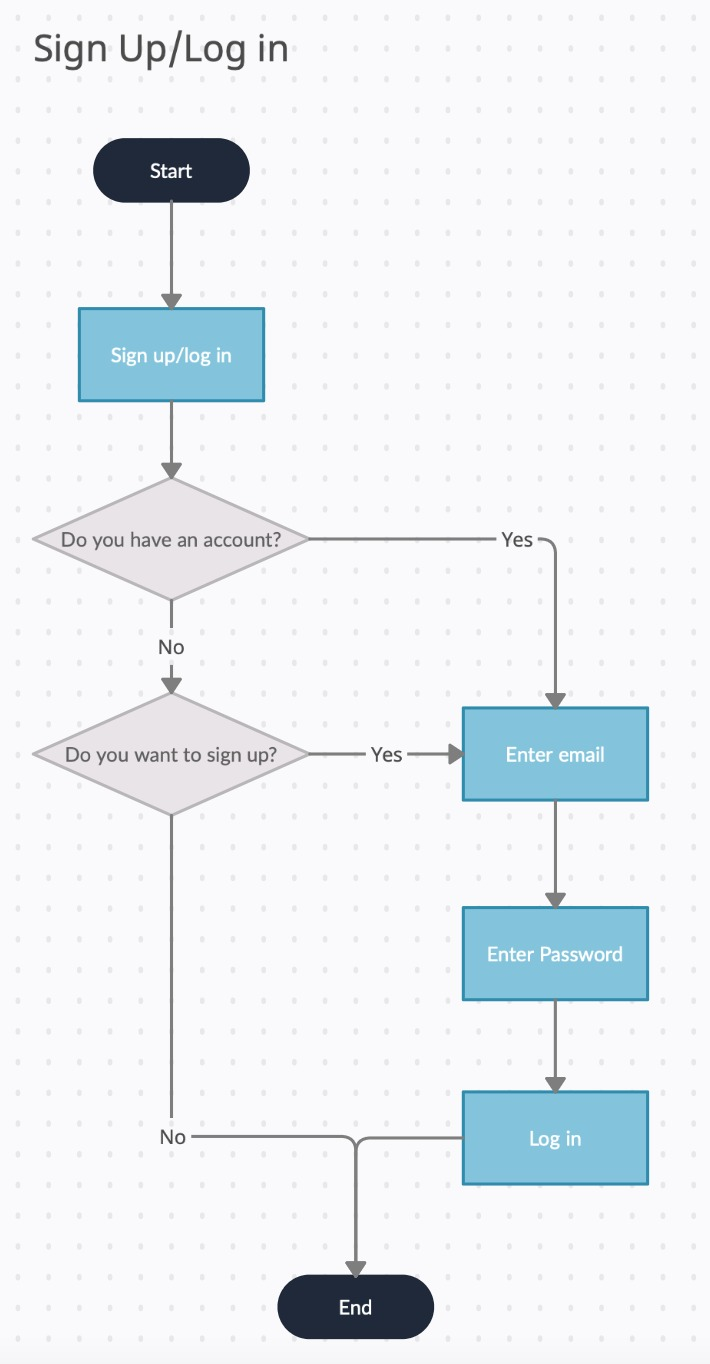
\includegraphics[height=65mm,scale=0.5]{Images/UseCase_Loggin.jpeg}}
            \caption{Signup/ Login Use Case}
            \label{fig}
        \end{figure} \\
    \item Connect to smart home: \\
       If the user creates a new account, the application will ask the user if they would like to connect their home devices. If the user logged in with their LG account and already have devices connected, the app will fetch the data from the LG application. 
        \begin{figure}[htbp]
            \centerline{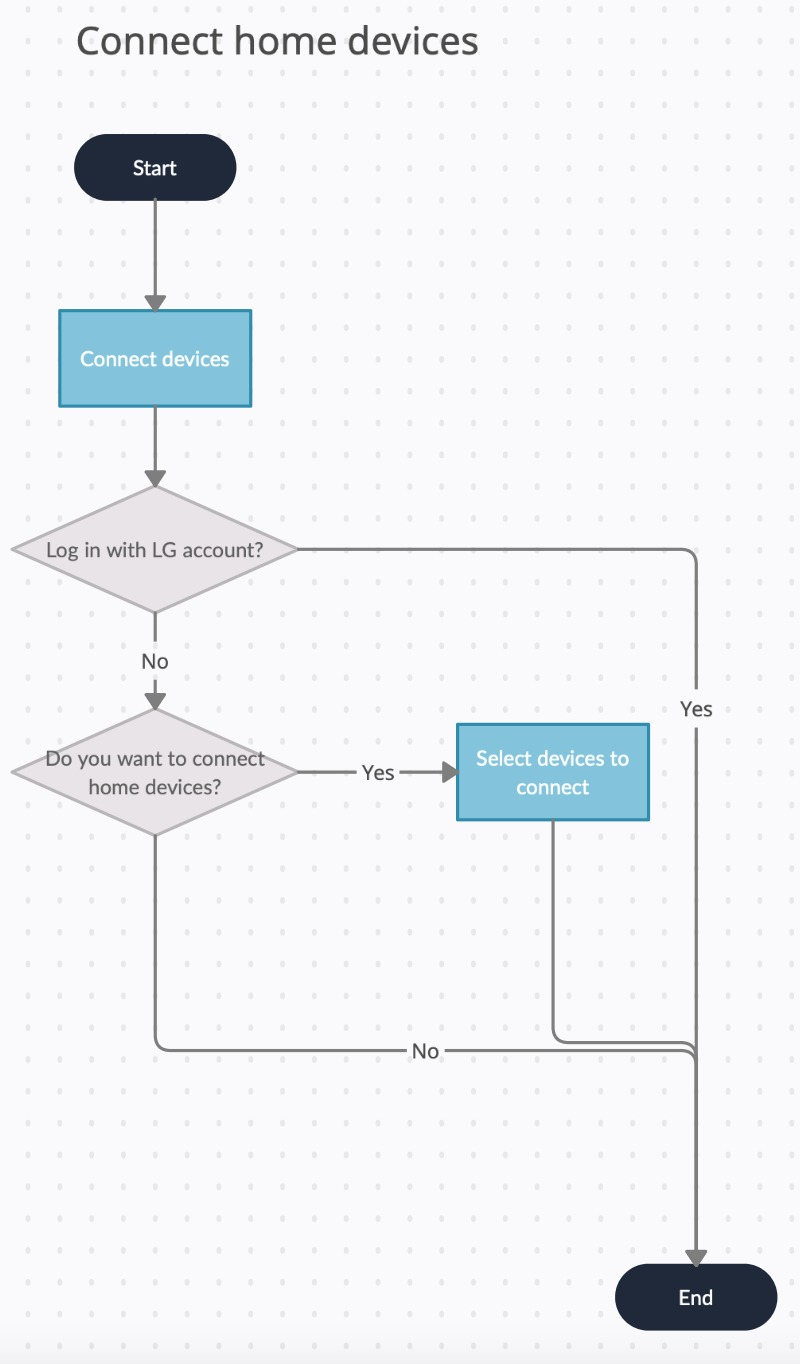
\includegraphics[height=65mm,scale=0.5]{Images/UseCase_ConnectHome.jpeg}}
            \caption{Connecting To Smart Home Use Case}
            \label{fig}
        \end{figure}\\
    \item Set alarm (from home screen) \\
       When a user wants to set a new alarm, they can do that from the home screen simply by pressing the plus in the upper right corner. If the user wants to set an already existing alarm, they can press the activation button on the alarm.
        \begin{figure}[htbp]
            \centerline{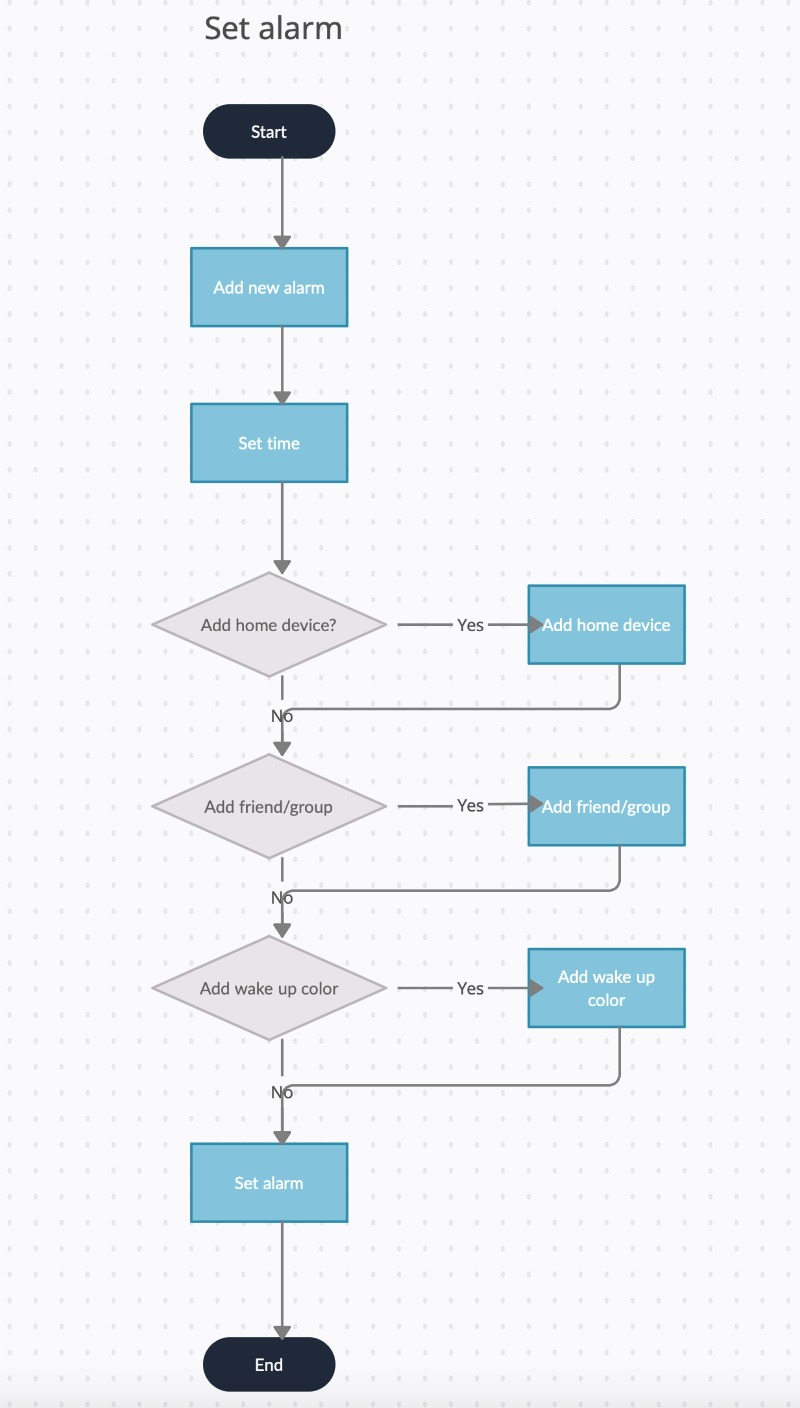
\includegraphics[height=65mm,scale=0.5]{Images/UseCase_SetAlarm.jpeg}}
            \caption{Set Alarm Use Case}
            \label{fig}
        \end{figure}\\
    \item Add Home Appliances \\
       In this page, the user can add their home appliances by clicking on the plus button. After adding appliances, they can be used to automate specific tasks while setting the alarm time. Also, multiple home appliances with their associated tasks can be grouped together into a favorite, customized program. 
        \begin{figure}[htbp]
            \centerline{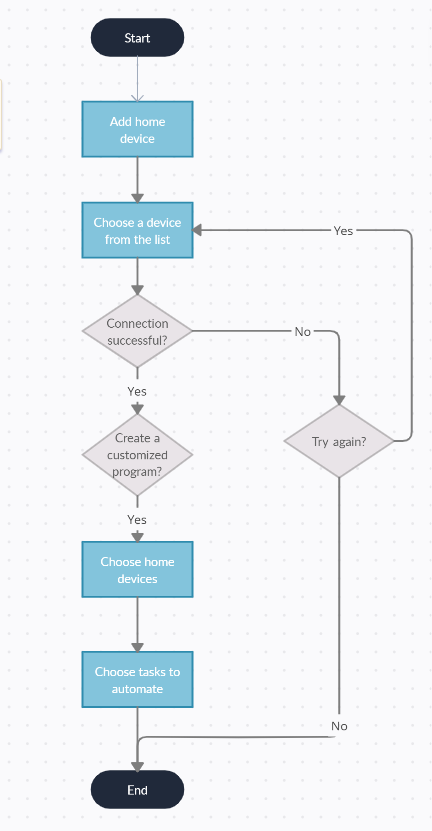
\includegraphics[height=75mm,scale=0.5]{Images/UseCase_ConnectDevice.png}}
            \caption{Adding Home Appliances Use Case}
            \label{fig}
        \end{figure}\\
    \item Add Friends \& Create Groups \\
       In order to add wake up buddies, the user has to search for friends and then send them a request. Besides, a user can select favorite friends or create a group.
        \begin{figure}[htbp]
            \centerline{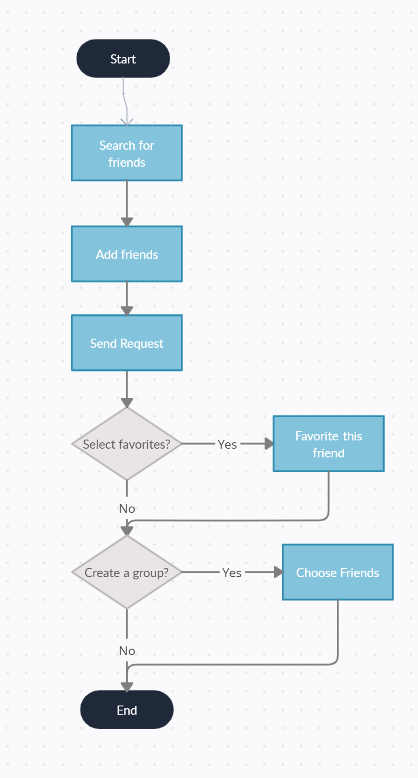
\includegraphics[height=75mm,scale=0.5]{Images/UseCase_AddFriend.png}}
            \caption{Adding Friends Use Case}
            \label{fig}
        \end{figure}\\
    \vspace{10pt}
    \item Change Settings \\
       In order to add wake up buddies, the user has to search for friends and then send them a request. Besides, a user can select favorite friends or create a group.
        \begin{figure}[htbp]
            \centerline{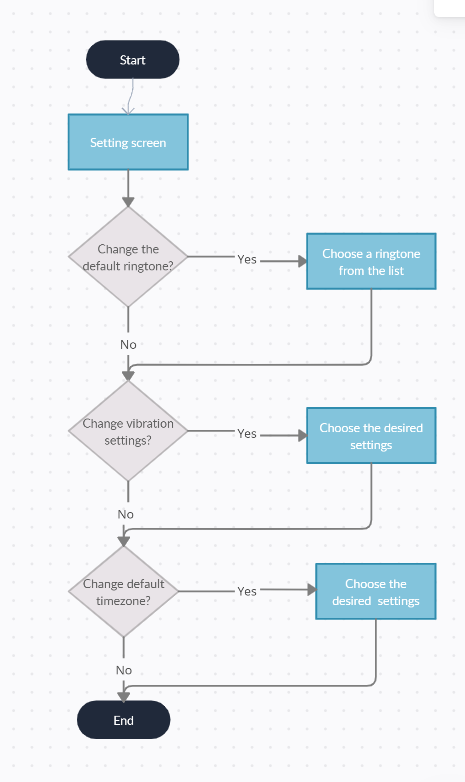
\includegraphics[height=75mm,scale=0.5]{Images/UseCase_Settings.png}}
            \caption{Changing Settings Use Case}
            \label{fig}
        \end{figure}\\
    
\end{enumerate}

\section{Discussion}
\par For all of us the project was a good experience. We all learned something new and also to work with people from all around the world was a good experience. Also, we learnt ow to create an App for Android using Kotlin. From a software engineering perspective, the team has successfully accomplished almost all steps  from market analysis, ideation, prototyping, and implementation p to the testing part of the development process. The team had regular meetings and ongoing check-ups on how the development was going. In the beginning, a lot of focus was on the project itself and it was similar to what was in line with the course. The further into the project we came, the more we started to shift focus into the development of the app itself and not so much on documentation, which is a major part in this course. In the end, the focus was once again shifted back to the documentation and creating good documentation. 
\par Now when we look back there were certainly things we underestimated or stuff we didn’t think through. Our time management also wasn’t on point throughout the project. We started too late with our implementation so it was quite a busy end for all of us. We also met every week if possible but for a next time it would be better to meet earlier in the week and not just the day before our lecture. Another mistake we made was in splitting the work. We could have split the work more into smaller tasks and work parallel. We used branches but it wasn’t really Agile.
\par For the future, we learnt that it would be useful to work on the coding tasks together in a room, especially during the early phases of development. This would make it easier to communicate in real time with each other and also get immediate feedback. Furthermore, it would help us bond as a team. We think this could have helped us much.

\end{document}



